\documentclass[preprint, 3p,
authoryear]{elsarticle} %review=doublespace preprint=single 5p=2 column
%%% Begin My package additions %%%%%%%%%%%%%%%%%%%

\usepackage[hyphens]{url}

  \journal{Neurocomputing} % Sets Journal name

\usepackage{graphicx}
%%%%%%%%%%%%%%%% end my additions to header

\usepackage[T1]{fontenc}
\usepackage{lmodern}
\usepackage{amssymb,amsmath}
% TODO: Currently lineno needs to be loaded after amsmath because of conflict
% https://github.com/latex-lineno/lineno/issues/5
\usepackage{lineno} % add
\usepackage{ifxetex,ifluatex}
\usepackage{fixltx2e} % provides \textsubscript
% use upquote if available, for straight quotes in verbatim environments
\IfFileExists{upquote.sty}{\usepackage{upquote}}{}
\ifnum 0\ifxetex 1\fi\ifluatex 1\fi=0 % if pdftex
  \usepackage[utf8]{inputenc}
\else % if luatex or xelatex
  \usepackage{fontspec}
  \ifxetex
    \usepackage{xltxtra,xunicode}
  \fi
  \defaultfontfeatures{Mapping=tex-text,Scale=MatchLowercase}
  \newcommand{\euro}{€}
\fi
% use microtype if available
\IfFileExists{microtype.sty}{\usepackage{microtype}}{}
\usepackage[]{natbib}
\bibliographystyle{plainnat}

\ifxetex
  \usepackage[setpagesize=false, % page size defined by xetex
              unicode=false, % unicode breaks when used with xetex
              xetex]{hyperref}
\else
  \usepackage[unicode=true]{hyperref}
\fi
\hypersetup{breaklinks=true,
            bookmarks=true,
            pdfauthor={},
            pdftitle={On time series features and forecasting by temporal aggregation},
            colorlinks=false,
            urlcolor=blue,
            linkcolor=magenta,
            pdfborder={0 0 0}}

\setcounter{secnumdepth}{5}
% Pandoc toggle for numbering sections (defaults to be off)


% tightlist command for lists without linebreak
\providecommand{\tightlist}{%
  \setlength{\itemsep}{0pt}\setlength{\parskip}{0pt}}



\usepackage{float}
\floatplacement{figure}{!htb}
\usepackage{algorithm}
\usepackage{algpseudocode}
\usepackage{enumitem}
\usepackage{pdflscape}
\newcommand{\blandscape}{\begin{landscape}}
\newcommand{\elandscape}{\end{landscape}}
\usepackage{booktabs}
\usepackage{longtable}
\usepackage{array}
\usepackage{multirow}
\usepackage{wrapfig}
\usepackage{float}
\usepackage{colortbl}
\usepackage{pdflscape}
\usepackage{tabu}
\usepackage{threeparttable}
\usepackage{threeparttablex}
\usepackage[normalem]{ulem}
\usepackage{makecell}
\usepackage{xcolor}



\begin{document}


\begin{frontmatter}

  \title{On time series features and forecasting by temporal
aggregation}
    \author[Cardiff Business School]{Bahman Rostami-Tabar%
  \corref{cor1}%
  }
   \ead{rostami-tabarb@cardiff.ac.uk} 
    \author[The Institute for Artificial Intelligence of Serbia]{Dejan
Mircetic%
  %
  \fnref{1}}
   \ead{dejan.mircetic@ivi.ac.rs} 
      \affiliation[Cardiff Business School]{Cardiff Business School, 3
Colum Drive, CF10 3EU, Cardif}
    \affiliation[The Institute for Artificial Intelligence of
Serbia]{Institute for Artificial Intelligence research and development
of Serbia, Fruskogorska 1, 21000 Novi Sad}
    \cortext[cor1]{Corresponding author}
    \fntext[1]{Equal contribution}
  
  \begin{abstract}
  When a forecast of the total value over a number of time periods ahead
  is required, forecasters are presented with two temporal aggregation
  (TA) approaches approaches to produce required forecasts: i)
  aggregated forecast (AF) or ii) aggregate data using non-overlapping
  temporal aggregation (AD). Often, the recommendation is to aggregate
  data to a frequency relevant to the decision the eventual forecasts
  will support and then produce the forecast. However, this might not be
  always the best choice and we argue that both AF and AD approaches may
  outperform each other in different situations. Moreover, there is a
  lack of evidence on what indicators may determine the superirity of
  each approach. We design and execute an empirical experiment framework
  to first explore the performance of these approaches using monthly
  time series of M4 competition dataset. We further turn the problem
  into a classification supervised learning and build a machine learning
  algorithm to investigate the connection between time series features
  and the performance of temporal aggregation. This is the first study
  in time series forecasting that explores the association between time
  series features and temporal aggreagtion performance. Our findings
  suggest that neither AF or AD approaches perform accurately for each
  individual series. AF is shown to be significantly better than AD for
  the monthly M4 time series, especially for longer horizons. We build
  several machine learning approaches using a set of extracted time
  series features as input to predict accurately whether AD or AF
  oshould be used. We find out Random Forest (RF) is the most accurate
  approach in correctly classifying the oucome examined both by
  staitical measures such as missclassification error, F-statistics, and
  area under the curve and a utility measure. The RF approach reveals
  that curvature, nonlinearity, seas\_pacf, unitroot\_up, mean,
  ARCHM.LM, Coifficient of Variation, stability, linearity and
  max\_level\_shif are among the most important features in driving the
  predictions of the model. Our findings indicate that the strength of
  trend, ARCH.LM, hurst, autocorrelation lag 1 and unitroot\_pp and
  seas\_pacf may favor AF approach, while lumpiness, entropy,
  nonlinearity, curvature, stremgth of seasonality may increase the
  chance of AD performing better. We conclude the study by sumamrising
  the finding and present an agenda for further research.
  \end{abstract}
    \begin{keyword}
    Temporal Aggregation \sep Forecasting \sep Time Series
Feature \sep Exponential Smoothing \sep Machine Learning \sep Random
Forest \sep 
    Classification
  \end{keyword}
  
 \end{frontmatter}

\hypertarget{introduction}{%
\section{Introduction}\label{introduction}}

Time series forecasting has been used for many decades to inform
decisions in various sectors such as business, finance, economy, supply
chain and healthcare \citep{petropoulos2022forecasting}. With advances
in technology, data can often be collected at the time of transaction or
service, e.g.~call arrival times in a call centre, point of sales in
retail, or incidents attended in an ambulance service. In electronic
databases, temporal data are generally stored in a single level of
granularity.

One common assumption in time series forecasting is that the time series
granularity matches the forecast requirement, i.e.~to produce daily
forecasts, we use daily time series. However, the level of time series
granularity does not necessarily match the level of forecast
granularity, driven by the decision-making process. Indeed, in practice
the level of temporal granularity in the forecast requirement is often
lower than the existing time series granularity. For instance, while a
forecast might be required at the annual (daily) level, the time series
is available at monthly (hourly) level. We also recognise that there
might be cases where forecast granularity is higher than the existing
series, however this requires introducing a disaggregation mechanism and
is not covered in this study.

Generally, forecast granularity level and its horizon are determined by
decisions made in the light of forecasts. In this paper, we consider a
situation where an original time series has a higher temporal
granularity (e.g.~monthly) than the required forecast (e.g.~annual). We
aim to generate a forecast of the total value over several time periods
ahead, which is referred to as forecast horizon aggregation or forecast
over the lead-time period \citep{mohammadipour2012forecast}. Therefore,
the lead-time period matches the aggregation level required to aggregate
the time series.

Producing an aggregated forecast over a number of periods is required in
many situations to inform decisions about capacity planning, inventory
management, logistics, procurement, and others
\citep{nikolopoulos2011aggregate, zotteri2007model}. For example,
generating a forecast for the whole lead-time period is often required
to determine the level of safety stock in inventory management. In an
emergency department, while the historical hourly time series of
admission is available, daily forecasts might be required for rostering,
while quarterly forecasts might be useful for resource planning
\citep{rostami2020anticipating}. In a supply chain, yearly forecasts
might be used for procurement and budgeting decisions, while the time
series might be available at a monthly granularity
\citep{mircetic2021forecasting}.

A key question then to be answered is: should the original time series
be used to \textcolor{blue}{generate} the forecast for the required
horizon and then sum them up to obtain the forecast over time periods
(lead-time), i.e.~Aggregate Forecast (AF)\textcolor{blue}{,} or should
we first aggregate the time series to match the forecast requirement
granularity and then extrapolate directly at that level, i.e.~Aggregate
Data (AD). This has been illustrated in Figure \ref{fig:example_oanoa}.

\begin{figure}[H]
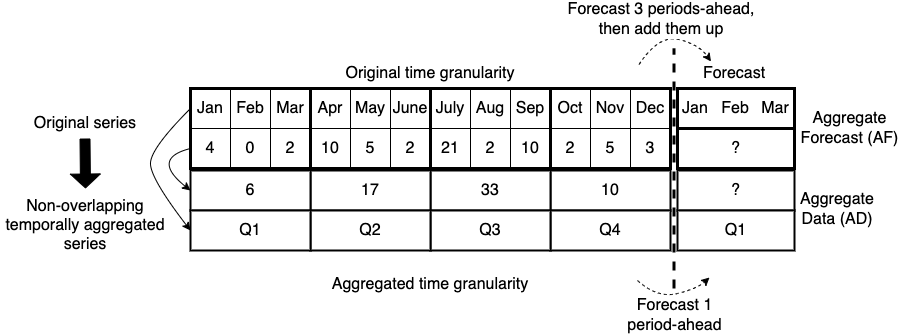
\includegraphics[width=0.9\linewidth]{img/300dpi/nota} \caption{Aggregate forecast vs. aggregate data approaches. Assuming a montly time series is available and a forecast over one quarter (aggregation level = 3 months) is required. We first generate forecast for 3 periods ahead and then sum them up to create forecast over the quarter (Forecast by AF approach). Then, we create the temporally aggregated series by dividing the original series into the block of 3 periods. Next, we forecast for 1 period ahead (Forecast by AD approach).}\label{fig:example_oanoa}
\end{figure}

For the later, we often use the non-overlapping temporal aggregation
(NOTA) approach. Using this approach, the original series is divided
into a consecutive non-overlapping bucket of time, starting from the
most recent period backward. The size of the bucket is equal to the
number of time periods required in forecasting, which is referred to
\textcolor{blue}{as aggregation level}, \(m\). The aggregated series is
then created by summing up the values inside each bucket. The number of
aggregate observations is \([N/m]\), where \(N\) is the number of
periods, and the \([x]\) operator returns the integer part of \(x\)
\citep{rostami2019impact}.
\textcolor{blue}{When we aggregate data to lower frequency domain such as annual using NOTA, we loose some information and AD is losing some of the sensitivity compared to AF. AF may better capture detailed information at the higher frequency resulting in better accuracy. However, this might be also affected by forecast horizon, as using AF might not be useful when forecasting far ahead into the future.}

There are some studies that investigate this question when considering
forecasting at one single level of aggregation
\citep{rostami2013demand, rostami2014note, kourentzes2017demand} or
forecast combinations using multiple temporal aggregation levels
\citep{kourentzes2014improving} or temporal hierarchies
\citep{athanasopoulos2017forecasting}. These approaches have been
applied \citep{nikolopoulos2011aggregate, petropoulos2014forecast} in
both intermittent demand \citep{nikolopoulos2021we} and fast-moving
demand contexts \citep{athanasopoulos2017forecasting}.

The overall conclusion is that both aggregate forecast and aggregate
data approaches may outperform each other. Their performance may depend
on the presence of the autocorrelation in the original series,
aggregation level, forecast horizon and the employed forecasting method
(see, e.g.,
\citet{boylan2016performance};\citet{rostami2021aggregate};\citet{rostami2014note};\citet{nikolopoulos2011aggregate}).
We should note that this study only applies to the case of a single
level of aggregation, we can extend this study to examine the case of
using multiple level of aggregation, temporal hierarchies or
multi-output forecast in the future.

\textcolor{blue}{Despite recent developments in this area, there is still a lack indications on which temporal aggregation approach should be used to forecast a time series, given its features. To our knowledge, this is the first study that explores the association between time series features and model performance in the context of forecasting by temporal aggregation (TA). The need for such research has also
been emphasised by @babai2022demand in a review article. This study contributes to the area of time series forecasting and intends to shed lights on how the performance of temporal aggregation approaches (i.e. both AF and AD) is associated with time series features. To that end, we use 48,000 time series from the monthly M4-competition dataset. First, we examine how the features of time series changes going from a high granularity level (e.g. monthly) to a low granularity (e.g. annual). We then build machine learning models to describe the association between the original time series features and the forecasting performance of temporal aggregation approaches. Next, we use models' outputs to discover which features are critical in predicting accurately the performance of temporal aggregation approaches, followed by an interpretation of features associated with the forecasting performance. This will help us to provide recommendations to forecasters and decision-makers on which approach to use.}

\textcolor{blue}{The research objectives are as following:}

\begin{enumerate}
\def\labelenumi{\arabic{enumi}.}
\item
  \textcolor{blue}{We measure 42 features of the time series at the original level (e.g. monthly) and at various levels of temporal aggregation (e.g. quarterly, annual) using the monthly M4 competition.}
\item
  \textcolor{blue}{We reveal how time series features change as we aggregate data from high frequency (e.g. monthly) to low frequency (e.g. annual).}
\item
  \textcolor{blue}{We assess the forecast accuracy performance of AD and AF approaches for the forecasts generated by the the Exponential Smoothing State Space (ETS) model.}
\item
  \textcolor{blue}{We build machine learning models using time series features as predictors to accurately predict which approach (AD or AF) performs better.}
\item
  \textcolor{blue}{We examine the association between time series features and the forecasting performance of these approaches.}
\end{enumerate}

The rest of the paper is organised as follows: section \ref{lit}
provides a brief overview of the use of temporal aggregation in time
series forecasting. Section \ref{framework} describes the empirical
experiment design, forecasting approaches, method and forecast accuracy
metrics. Section \ref{tsfeatures} describes time series features and
presents the time series features for monthly M4 competition dataset,
followed by analysing how non-overlapping temporal aggregation affects
time series features. We then examine the forecasting performance of AD
and AF approaches. Section \ref{ml} presents machine learning algorithms
and their performance on accurately classifying the performance of AD
and AF for a given time series and its features. Section \ref{res}
presents the important features and their connection with the
performance of temporal aggregation approaches. Section \ref{con}
provides concluding remarks and an agenda for future research.

\hypertarget{lit}{%
\section{Research background}\label{lit}}

In practice, a time series is generally stored at a single level of time
granularity. When the time series is available at a higher level of
granularity (e.g.~hourly), it is often expected to generate a forecast
at a lower granularity level (e.g.~daily) over several time periods.
Therefore, a forecast of the total value over several time periods ahead
(i.e.~lead-time or aggregation level) is required
\citep{mohammadipour2012forecast}. In these situations, an obvious
option, that is often recommended in practice \citep{goodwin2018profit},
would be to first transform the higher granularity time series into the
lower granularity that matches the forecast requirement, and then
produce the forecast. The transformation is generally performed using
non-overlapping temporal aggregation.

Another approach is to aggregate forecast rather than data. In that
case, we first produce forecasts using the higher granular time series
for the forecast horizon (i.e.~multiple periods ahead) and then
aggregate them.

The application of NOTA approach in time series forecasting has been
initially studied in the econometric literature. They evaluated how NOTA
may change the structure of Autoregressive Integrated Moving Average
(ARIMA) processes \citep{wei1978some, rossana1995temporal}. This
literature is in favor of aggregate data using NOTA. They show that it
leads to accuracy gains under the assumption of ARIMA process and using
an optimal conditional mean forecast.

\citet{rostami2013demand} and \citet{rostami2014note} further explored
analytically the effect of NOTA on forecasting performance at both
aggregated forecast horizon ( lead-time) and the disaggregated level
using Mean Squared Error (MSE). They assume that Single Exponential
Smoothing (SES) forecasting method is applied to an ARIMA(1,1) time
series. They determine the conditions under which aggregate data
outperforms the aggregate forecast approach. They show that the
superiority of each approach depends on the process parameters that are
affecting the time series features, parameters of the forecasting
method, and aggregation levels. They concluded that NOTA performs better
when autocorrelation is not highly positive. In contrast, they show that
high positive autocorrelation as one of the key features of time series,
favorites AF approach. \citet{rostami2019impact} evaluated the impact of
NOTA on forecasting demand and orders in a supply chain. They assume
that the demand time series follows an ARMA(1,1), the stock policy is
order-up-to-level and optimal forecasting is used to produce forecasts.
They showed that although the NOTA does not lead to an accuracy
improvement in terms of MSE at the retailer's level, however it can lead
to MSE reduction at the manufacturer level and a reduction of the
bullwhip effect.

\citet{mohammadipour2012forecast} also assessed analytically the effect
of temporal aggregation when the time series process is integer
autoregressive moving average, INARMA(\(p,q\)), processes. They
demonstrated that aggregate data leads to lower MSE compared to
aggregate forecast approach when the value of the autoregressive
parameter is high.

The potential forecasting benefit of TA was investigated by
\citet{willemain1994forecasting} and \citet{nikolopoulos2011aggregate}
in the context of intermittent time series.
\citet{willemain1994forecasting} empirically compared the forecast
accuracy improvement of AF and AD approaches. They showed that
aggregating time series can lead to more accurate forecasts.
\citet{nikolopoulos2011aggregate} showed that NOTA approach may offer
considerable improvements in terms of forecast accuracy. Further studies
\citep{babai2012impact, petropoulos2015forecast, kourentzes2014improving, spithourakis2011improving}
confirmed empirically the forecast and stock control improvement
resulted from NOTA. These studies covered both intermittent and fast
moving time series.

\citet{athanasopoulos2011tourism} investigated the benefits of aggregate
forecast versus aggregate data in an empirical study consisting of 366
monthly series and various forecasting methods including state space
models for exponential smoothing (ETS), ARIMA, and Theta. Their findings
are in favor of aggregating forecasts. They found that aggregating
forecast from either monthly or quarterly to yearly leads to more
forecast accuracy improvements than yearly forecasts generated from the
NOTA yearly series. Using time series of order and point-of-sale in a
retail supply chain, \citet{jin2015forecasting} assessed the benefits of
NOTA for forecast accuracy. They found that NOTA leads to more accurate
forecasts when the autocorrelation of time series is not highly
positive. In a study where a high frequency time series is used,
\citet{luna2011top} showed that in daily forecast of cash withdrawals,
NOTA results in similar or more accurate forecast than using hourly
series.

Some studies have investigated the benefits of producing forecasts using
multiple time series resulted from NOTA approach, corresponding to
multiple levels of aggregation. Forecasts are generated at each level
and then combined to obtain the required forecast.
\citet{kourentzes2014improving} recommended using multiple levels of
aggregation and combining the separate forecasts (MAPA). Multiple
studies in intermittent time series forecasting, promotional modeling
and inventory management highlighted the gain of using multiple TA
levels
\citep{petropoulos2014forecast, kourentzes2015forecasting, barrow2016distributions}.
\citet{athanasopoulos2017forecasting} proposed Temporal Hierarchies
Forecasting (THieF), which creates multiple temporally aggregated series
using NOTA, generate forecasts and then reconciles them to obtain the
required forecast.

\textcolor{blue}{A stream of research investigates the use of features in time series forecasting based on multiple time frequency spaces in visibility graphs. @liu2020fuzzy proposed a multiple time-frequency spaces fuzzy interval forecasting model using datasets from energy and finance. The original series is decomposed into different components, which are then used to reconstruct a group of time series at different temporal scales. Next, a prediction interval forecast is generated for the different reconstructed time series that are then aggregated using the induced-ordered weighted averaging aggregation operation to generate the final forecast. @hu2022efficient suggested a novel time series forecasting model based on a new metric measuring nodes similarity in visibility graph. In the proposed model, time series is first converted into a visibility graph. Next, similarities between nodes are determined and finally forecasts are generated using the normalized similarity distribution. @hu2022time investigated the features of time series to generate accuracy forecasts from the perspective of fuzzy interaction between nodes. They used a fuzzy cognitive visibility graph to convert the time series into a pair of directed weighted graphs. Then, the weighted multi-subgraph similarity is developed to calculate the similarity between nodes. They then proposed a novel forecasting method for time series forecasts based on fuzzy similarity distribution that can efficiently capture the spatio-temporal dependency in the time series data. The empirical results confirmed the benefits of leveraging fuzzy interaction for time series forecasting based on the visibility graphs.}

Although all approaches including AF, AD and using multiple TA levels
have demonstrated forecasting gain, arguably none of them are suitable
to be used in every situation. Almost all studies in the literature
reports an overall accuracy (e.g.~average) rather than accuracy at the
time series level). We argue that some time series features may favorite
using a particular approach over others. However, there is no study in
the literature that investigates the potential association between time
series features and temporal aggregation performance, which is the main
aim of this study.

\hypertarget{framework}{%
\section{Experiment framework}\label{framework}}

In this section, we describe the design of the empirical experiment used
in this study.
\textcolor{blue}{We first present the study framework, then describe AD and AF approaches and the ETS forecasting method, followed by forecasting error metrics.}

Figure \ref{fig:expdes} illustrates the framework of the experimental
design performed in this study. The framework consists of several steps
which are described as follows:

\begin{enumerate}
\def\labelenumi{\arabic{enumi}.}
\item
  \textcolor{blue}{The original monthly time series is transformed into temporally aggregated series for a given aggregation aggregation level, $m$.}
\item
  \textcolor{blue}{The ETS forecasting method is applied to the original series to generate forecast for $m$ periods.}
\item
  \textcolor{blue}{Forecasts are generated using ETS model for temporally aggregated series (forecasts from AD).}
\item
  Forecasts per each period are added up to obtain the forecast over the
  aggregated horizon (forecasts from AF).
\item
  Forecasts are generated for temporally aggregated series (forecasts
  from AD).
\item
  Forecast accuracy is calculated for each series.
\item
  A database consisting of time series features and the performance of
  the AF and AD approaches is constructed. Time series features are used
  as an input (predictors) and the winning approach (labeled as AF or AD
  based on the minimum error metric) creates the response variable.
\item
  Several machine learning (ML) models are built to accurately predict
  the superiority of AF/AD approaches using the data created in step 7.
  \textcolor{blue}{These models include: 1) Logistic regression (LR), 2) Linear discriminant analysis (LDA), 3) Quadratic discriminant analysis (QDA), 4) K-Nearest Neighbors (KNN), 5) Lasso, 6) Generalised Additive Model (GAM), 7) Boosting, 8) Support Vector Machine (SVM), 9) Random Forest (RF), 10) Google Brain TensorFlow model (TensorFlow), 11) Facebook's Deep learning Torch model based on tensors \& neural networks (DL Torch), 12) extreme gradient boosting (XGBoost), 13) recurrent neural network (RNN), 14) convolution neural network (CNN), 15) feedforward neural network (FNN) and 16) Dynamic Time Warping (DTW).}
  Researchers are referred to \citet{james2021statistical} for a detail
  description of these approaches. Given the outperformance of the
  random forest among all models used in this study, we will describe it
  in more details in section \ref{ml}.
\end{enumerate}

The model can help us to identify the most important time series
features that lead to the outperformance of RF. Moreover, it can also
reveal how time series features are connected to the performance of AD
and AF.

Due to the page restrictions, details regarding the initial set up,
method of optimization and cost function of these algorithms are not
presented in the paper, however they are available by request from the
authors. The experiment has been conducted in R software, and the
authors are willing to share the code for reproducibility.

\begin{figure}[H]

{\centering 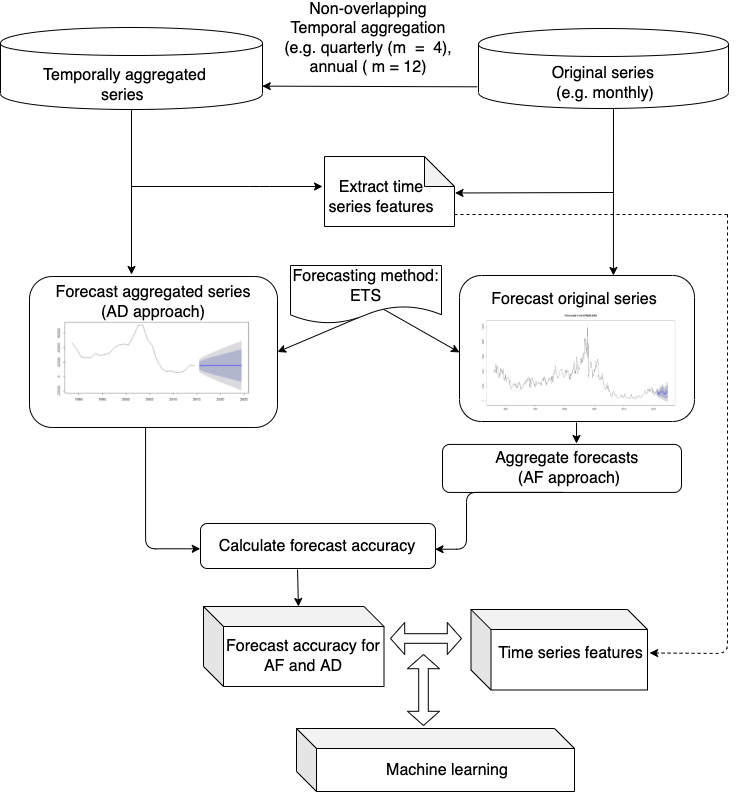
\includegraphics[width=0.7\linewidth]{img/300dpi/experiment_design} 

}

\caption{Design of the experiment framework}\label{fig:expdes}
\end{figure}

\hypertarget{forecasting-approaches}{%
\subsection{Forecasting approaches}\label{forecasting-approaches}}

We consider two different approaches to produce the forecast horizon
aggregation (i.e.~lead-time). Given that the original time granularity
is monthly, we aim at generating forecasts for various aggregation
levels that corresponds to 2-monthly (m = 2), quarterly (m = 3),
4-monthly (m = 4), semi-annual (m = 6) and annual (m = 12) time
granularity.

The first approach is to aggregate forecasts (AF).
\textcolor{blue}{This approach first involves generating base forecasts for $m$ periods ahead. Base forecasts are then aggregated to create forecasts at the aggregation horizon level.}
The main advantage of AF is that there is no loss of information from
the data because initial base forecasts are generated at the lowest
disaggregated level. AF approach can capture the dynamics of the high
frequency series, however they may be noisy and difficult to model. In
the case of stationary time series, the AF approach may produce a more
accurate forecast when the autocorrelation of the underlying demand
series is highly positive \citep{rostami2014note}. Conversely, there is
an absence of researches in the case of non-stationary time series.
Therefore, this research is dealing with both stationary and
non-stationary time series and provides insight into the perplexity of
interactions between different factors that influence on AF approach.

The second approach is to aggregate data (AD). This approach consists of
applying the non-overlapping temporal aggregation approach to the
original series, using the time granularity level for which the
forecasting is needed. Following that the process of forecasting the
temporally aggregated series for one atep ahead is performed. Benefits
of AD can be seen in the reduction of the noise in the data, as well as
in revelling the more smooth patterns that exist in the series. The NOTA
of the series usually sheds light on the key time series features, which
are more notable and clearer as we perform the aggregation to the lower
granularity levels (e.g.~quarterly, annual).

\hypertarget{forecasting-method}{%
\subsection{Forecasting method}\label{forecasting-method}}

The exponential smoothing state space (ETS) models
\citep{hyndman2021forecasting} are used to produce out of sample
forecasts, although our experiment design is model agnostic and could be
expanded to any other forecasting model. ETS can capture trend,
seasonality and error components in a time series through various forms
such as additive, multiplicative or mixed. ETS accounts for 18 different
exponential smoothing models. The automatic exponential smoothing model
is used using \emph{ets()} function in the forecast package
\citep{hyndman2008automatic} in R to produce forecasts for the original
and aggregated time series. For each series, \emph{ets()} identifies the
most accurate model using the corrected Akaike's Information Criterion
(AICc). Using an automatic forecasting method such as ETS is suitable
for this study, as we can assume that the best model is selected for
each series and this may help to separate the effect of the applied
forecasting method from TA approaches (i.e.~AF and AD).

\hypertarget{errormetric}{%
\subsection{Forecast accuracy measures}\label{errormetric}}

In this experiment, forecast accuracy evaluation is required at two
different stages. We first use an error metric (e.g.~Root Mean Squared
Scaled Error) to quantify the forecast accuracy of AF and AD in
generating time series forecast over lead-time for each time series and
ETS method. We consider the in-sample and the out-of-sample sets in
monthly M4 competition time series. We apply the ETS method to each
series in the in-sample dataset and keep their forecast for the
out-of-sample using time series cross validation with re-estimation. The
forecast horizon for the original time series equals \(m\), the
aggregation level, and the horizon for non-overlapping aggregated series
is one. We then compute the forecast errors over the test period of each
time series. To evaluate the forecast accuracy and bias, several
measures including Root Mean Squared Error (RMSE), Mean Absolute Error
(MAE) and Mean Error (ME), Mean Absolute Percentage Error (MAPE), Mean
Absolute Scaled Error (MASE) and Root Mean Squared Scaled Error (RMSSE)
are used.
\textcolor{blue}{We only present the results for RMSSE due to the space limit of the journal and also because it is the recommended error metric in M5 competition [@M5competition2022]. We share the R code and the Rmarkdown file through the GitHub repository, which provide the possibility of changing the error metric in the YAML section of the Rmarkdown to obtain results for other metrics. We should also note that similar conclusions are reached when using other accuracy metrics.}

RMSSE is given by:

\[ \text{RMSSE} = \sqrt{\text{mean}(q_{j}^2)},\]

where

\[q^2_{j} = \frac{\displaystyle e^2_{j}}
    {\displaystyle\frac{1}{T-m}\sum_{t=m+1}^T (y_{t}-y_{t-m})^2},\]

\textcolor{blue}{where $e_{j}$ is the forecast error, the difference between an observed value and its forecast. $y_{t}$ is an observed value at period $t$, $T$ is the length of time series, and $m$ is the seasonal length (e.g. for monthly m=12. For non-seasonal data, $m=1$.}

Second, we need to report how accurately a classification model predicts
the outcome (i.e.~the most accurate approach labeled as AF and AD), when
presented with a set of time series features at the original series. To
that end, we report several statistical measures including
misclassification error, F-statistics and area under the curve (AUC).

The misclassification error is calculated as following:

\[Misclassification_{error} = 100\% \times \left( 1-\frac{(t_p+t_n)}{N}\right),\]

\textcolor{blue}{where $N$ is the total number of cases to predict, $t_p$ is the true positive (i.e. when the model correctly predicts the outperformance of AF approach over AD) and $t_n$ is true negative (i.e. when the model correctly predicts the underperformance of AF approach over AD).}

F statistic is defined as:

\[F_{statistics} = 2 \times 100\% \times \left(\frac{(t_p/(t_p+f_p) \times t_p/(t_p+f_n))}{(t_p/(t_p+f_p)+t_p/(t_p+f_n)}\right),\]

Where \(f_p\) is false positive and \(f_n\) is false negative.

\textcolor{blue}{The false positive rate represents the fraction of cases in which AD was incorrectly classified as a right model to use, while the AF was the correct one. Similarly, the false negative rate represents the fraction of cases in which AF was incorrectly classified as a right model to use, while AD was the correct one.}

\textcolor{blue}{We can also illustrate the trade-off between false positives and true positives using a curve. It is called a receiver operating characteristic curve, or ROC curve [@james2021statistical]. The ROC curve is a plot of the true positive rate ($t_p$, sensitivity) versus the false positive rate ($f_p$, 1 - specificity) for a set of thresholds. We can quantify this by calculating the area under the curve, or AUC. The higher AUC, the better the model does at predictions. The maximum value of AUC is 1, which would be considered as a perfect prediction. Conversely, a model that performs no better than chance will have an AUC of 0.5 and would be considered as a poor one.}

In addition to the statistical measures discussed above, we also perform
the utility evaluation of different models. The utility metric
approximates the costs and benefit of wrong and correct classification.
For that purpose, average RMSSE error is used as a utility metric.

To assess the prediction accuracy of models, we split the data created
in the step 7 of Section \ref{framework} into a training and a test set.
To that end, we randomly divided the data on train and test set in a
\(70/30 \%\) split. The train data (33600 cases) is used for training
different algorithms, while the test data (14400 cases) is used to
evaluate the performance of models.

\hypertarget{tsfeatures}{%
\section{Time series data, features and temporal aggregation
performance}\label{tsfeatures}}

In this section, we first introduce the time series features extracted
for each time series. Following that, we \textcolor{blue}{illustrate}
these features for the monthly M4 competition dataset. Then, we describe
how non-overlapping temporal aggregation changes these features.
Finally, we discuss the forecasting performance of AD and AF applied to
the monthly M4 dataset.

\hypertarget{time-series-features}{%
\subsection{Time series features}\label{time-series-features}}

Table \ref{tab:summaryfeature} presents the description of features used
in this study. For each time series (original or aggregated), we compute
a set of measures from the training data. These features are also
described in detail by \citet{wang2009rule}, \citet{hyndman2015large}
and \citet{hyndman2021forecasting}.

\textcolor{blue}{Given the complexity of the relationship between the time series features and the performance of temporal aggregation approaches, we have considered all 42 features as predictor rather than using only few limited numbers of features known to users such as the strength of trend or seasonality, to develop an accurate prediction model. Using a reduced number of features either selected based on their interpretability or using dimensional reduction techniques might reduce the predictability power of the model, but this could be an interesting avenue for future research.}

\begin{table}[!h]

\caption{\label{tab:summaryfeature}     extcolor{blue}{Time series features considered in this study and their descriptions} }
\centering
\resizebox{\linewidth}{!}{
\fontsize{11}{13}\selectfont
\begin{tabular}[t]{ll}
\toprule
Feature & Description\\
\midrule
mean & Mean\\
var & Variance\\
cv & Coefficient of variation\\
trend & Strength of trend, a value close to 1 indicate highly trended series\\
seasonal\_strength & Strength of seasonality, a value close to 1 indicate highly seaonal series\\
entropy & Measure of how easy the series is to forecast. Entropy close to 0 shows a series  is easy to forecast\\
lumpiness & Lumpiness is the variance of the variances of  tiled (non-overlapping) windows\\
flat\_spots & Number of sections of the data where the series is relatively unchanging\\
crossing\_points & Number of times a time series crosses the median\\
nonlinearity & Extent of nonlinearity, if values around 0  series is linear. Large values shows nonlinearity\\
stability & Stability is the variance of the means of  tiled (non-overlapping) windows\\
hurst & Hurst coefficient of a time series which is a measure of long memory\\
spike & Prevalence of spikes in the remainder component  of the STL decomposition\\
linearity & Linearity of the trend component of the STL decomposition\\
curvature & Curvature of the trend component of the STL decomposition\\
peak & Timing of the peaks\\
trough & Timing of the troughs\\
x\_acf1 & First autocorrelation coefficient\\
x\_acf10 & Sum of squares of the first ten autocorrelation coefficients\\
diff1\_acf1 & First autocorrelation coefficient from the differenced series\\
diff1\_acf10 & Sum of squares of the first ten autocorrelation coefficients from the differenced series\\
diff2\_acf1 & First autocorrelation coefficient from the twice differenced data\\
diff2\_acf10 & Sum of squares of the first ten autocorrelation coefficients from the twice differenced series\\
seas\_acf1 & Autocorrelation coefficient at the first seasonal lag\\
x\_pacf5 & Sum of squares of the first 5 partial autocorrelation coefficients\\
diff1x\_pacf5 & Sum of squares of the first 5 partial autocorrelation coefficients of differenced series\\
diff2x\_pacf5 & Sum of squares of the first 5 partial autocorrelation coefficients of second-order differenced\\
seas\_pacf & Partial autocorrelation coefficient at the first seasonal lag\\
unitroot\_kpss & Kwiatkowski-Phillips-Schmidt-Shin (KPSS) test\\
unitroot\_pp & Phillips-Perron statistic for testing if a series is non-stationary\\
arch\_acf & Sum of squares of the first 12 autocorrelations of squared series\\
garch\_acf & Sum of squares of the first 12 autocorrelations of residuals, after fitting an GARCH(1,1)\\
arch\_r2 & R2 value of an AR model applied to the squared series\\
garch\_r2 & R2 value of an AR model applied to  residuals, after fitting an GARCH(1,1)\\
ARCH.LM & Statistic based on the Lagrange Multiplier (LM) test  for autoregressive conditional heteroscedasticity (ARCH)\\
e\_acf1 & First autocorrelation coefficient of the remainder series\\
e\_acf10 & Sum of squares of the first ten autocorrelation coefficients of the remainder series\\
max\_level\_shift & Largest mean shift between two consecutive sliding windows of the time series\\
time\_level\_shift & Timing index of the largest mean shift between two consecutive sliding windows of the time series\\
max\_var\_shift & Largest variance shift between two consecutive sliding windows of the time series\\
time\_var\_shift & Timing index of the largest variance shift between two consecutive sliding windows of the time series\\
\bottomrule
\end{tabular}}
\end{table}

\hypertarget{mtsmeasure}{%
\subsection{Time series features of monthly M4 data}\label{mtsmeasure}}

We use the monthly M4 competition time series to empirically examine the
performance of AD and AF and investigate the connection between their
performance and time series features. The monthly M4 data contains
48,000 time series from the Economic, Finance, Demographics and Industry
areas, while also including data from Tourism, Trade, Labor and Wage,
Real Estate, Transportation, Natural Resources and the Environment
\citep{Makridakis2018}. The monthly data is the most important data for
the business applications \citep{Spiliotis2020} and therefore the
largest class in M4, containing almost half of the data (48000 time
series).

For each time series in the monthly M4 dataset, we extract 41 features
as described in Table \ref{tab:summaryfeature} using \emph{tsfeatue()}
function in the tsfeatures package in R \citep{tsfeatures2020}.
Additionally, we include one more feature defined as origin, which is
the origin of the time series M4 competition data, i.e.~Economic,
Finance, Demographics and Industry.

Figure \ref{fig:feature1} and \ref{fig:feature2} illustrates the
corresponding distribution of each feature. Y-axis shows the frequency
in terms of the number of time series, and X-axis indicates the range of
values extracted for each feature. These figures show that the monthly
M4 data covers a wide range of time series features, which makes it a
suitable dataset for this research problem. We describe some significant
features observed in the dataset, and readers are referred to Figure
\ref{fig:feature1} and \ref{fig:feature2} for a full illustration of the
features.

The spectral entropy plot indicates that there is a range of time series
from easy (less noise, more systematic information) to hard (more noise,
less systematic information) to forecast. Coefficient of Variation is
also skewed to the right and indicates less variability for the majority
of series. The trend peaks near one and is skewed to the right
indicating the strong presence of the trend in this dataset. We also
observe that the nonlinearity feature peaks near zero and it is skewed
to the right, which indicates the lack of nonlinearity in the time
series. The autocorrelation lag1 and seasonal autocorrelation lag1 is
skewed to the left, and is highly positive for many time series. We also
measure the seasonal autocorrelation lag1 which is highly positive.
Lumpiness is extremely low for almost all time series and stability has
a range from low to high values. Both seasonal partial autocorrelation
and the strength of seasonality indicate a lower strength of
seasonality. Both stationaity and non-stattioanirity of series are
measured using unitroot\_pp and unitroot\_kpss statistics. They indicate
a strong presence of staitonairy time series. Curvature shows a sharp
distribution centered around zero, which means that most series do not
have stochastic or chaotic nature. Time series of stochastic nature are
associated with curves displaying positive curvature in a neighborhood
of their initial points, whereas curves related to chaotic phenomena
have a negative curvature. Hurst has a left skewed distribution with
almost all series with a value close to one indicating the presence of
the long memory in the series, which is related to the autocorrelation.

The distribution of the e\_acf10 values is skewed to right and the plot
shows that for most of the time series e\_acf10 is close to zero, which
means the leftover from trend and seasonality seems to be random.

\begin{figure}[H]

{\centering 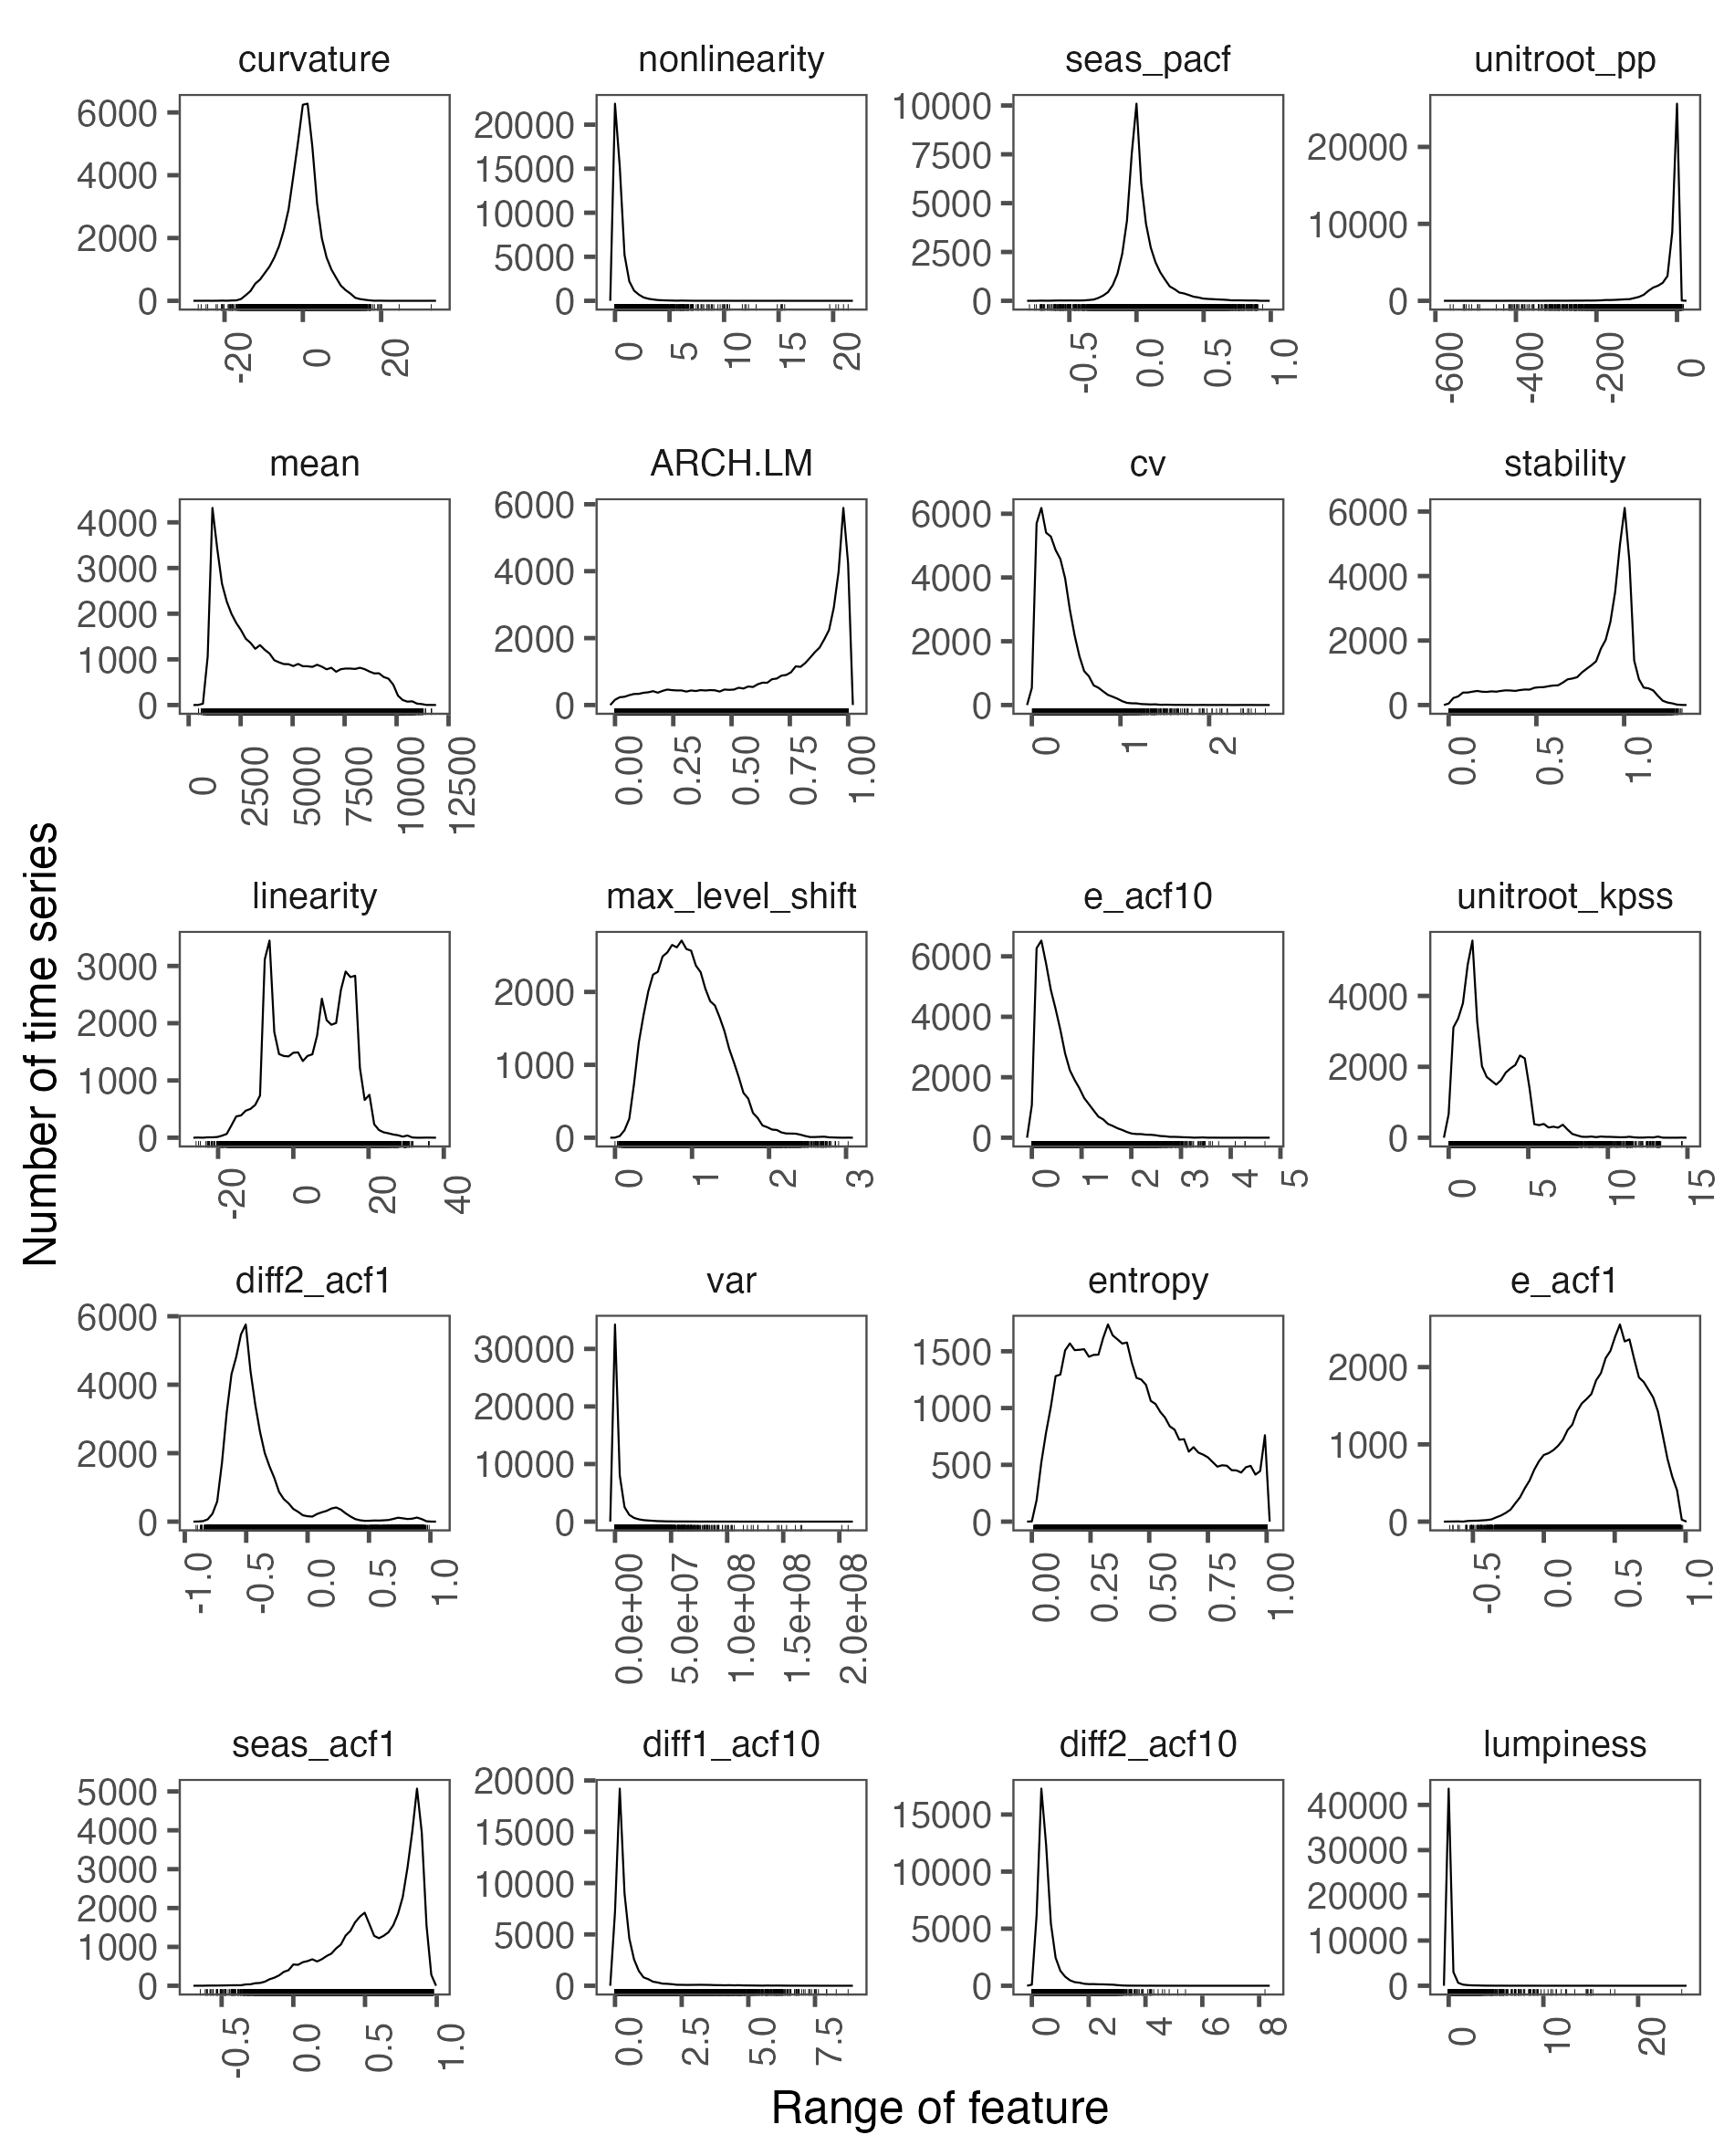
\includegraphics[width=0.7\linewidth]{img/300dpi/featurets_selection1} 

}

\caption{   extcolor{blue}{Features of monthly time series from M4 competition dataset} }\label{fig:feature1}
\end{figure}

\begin{figure}[H]

{\centering 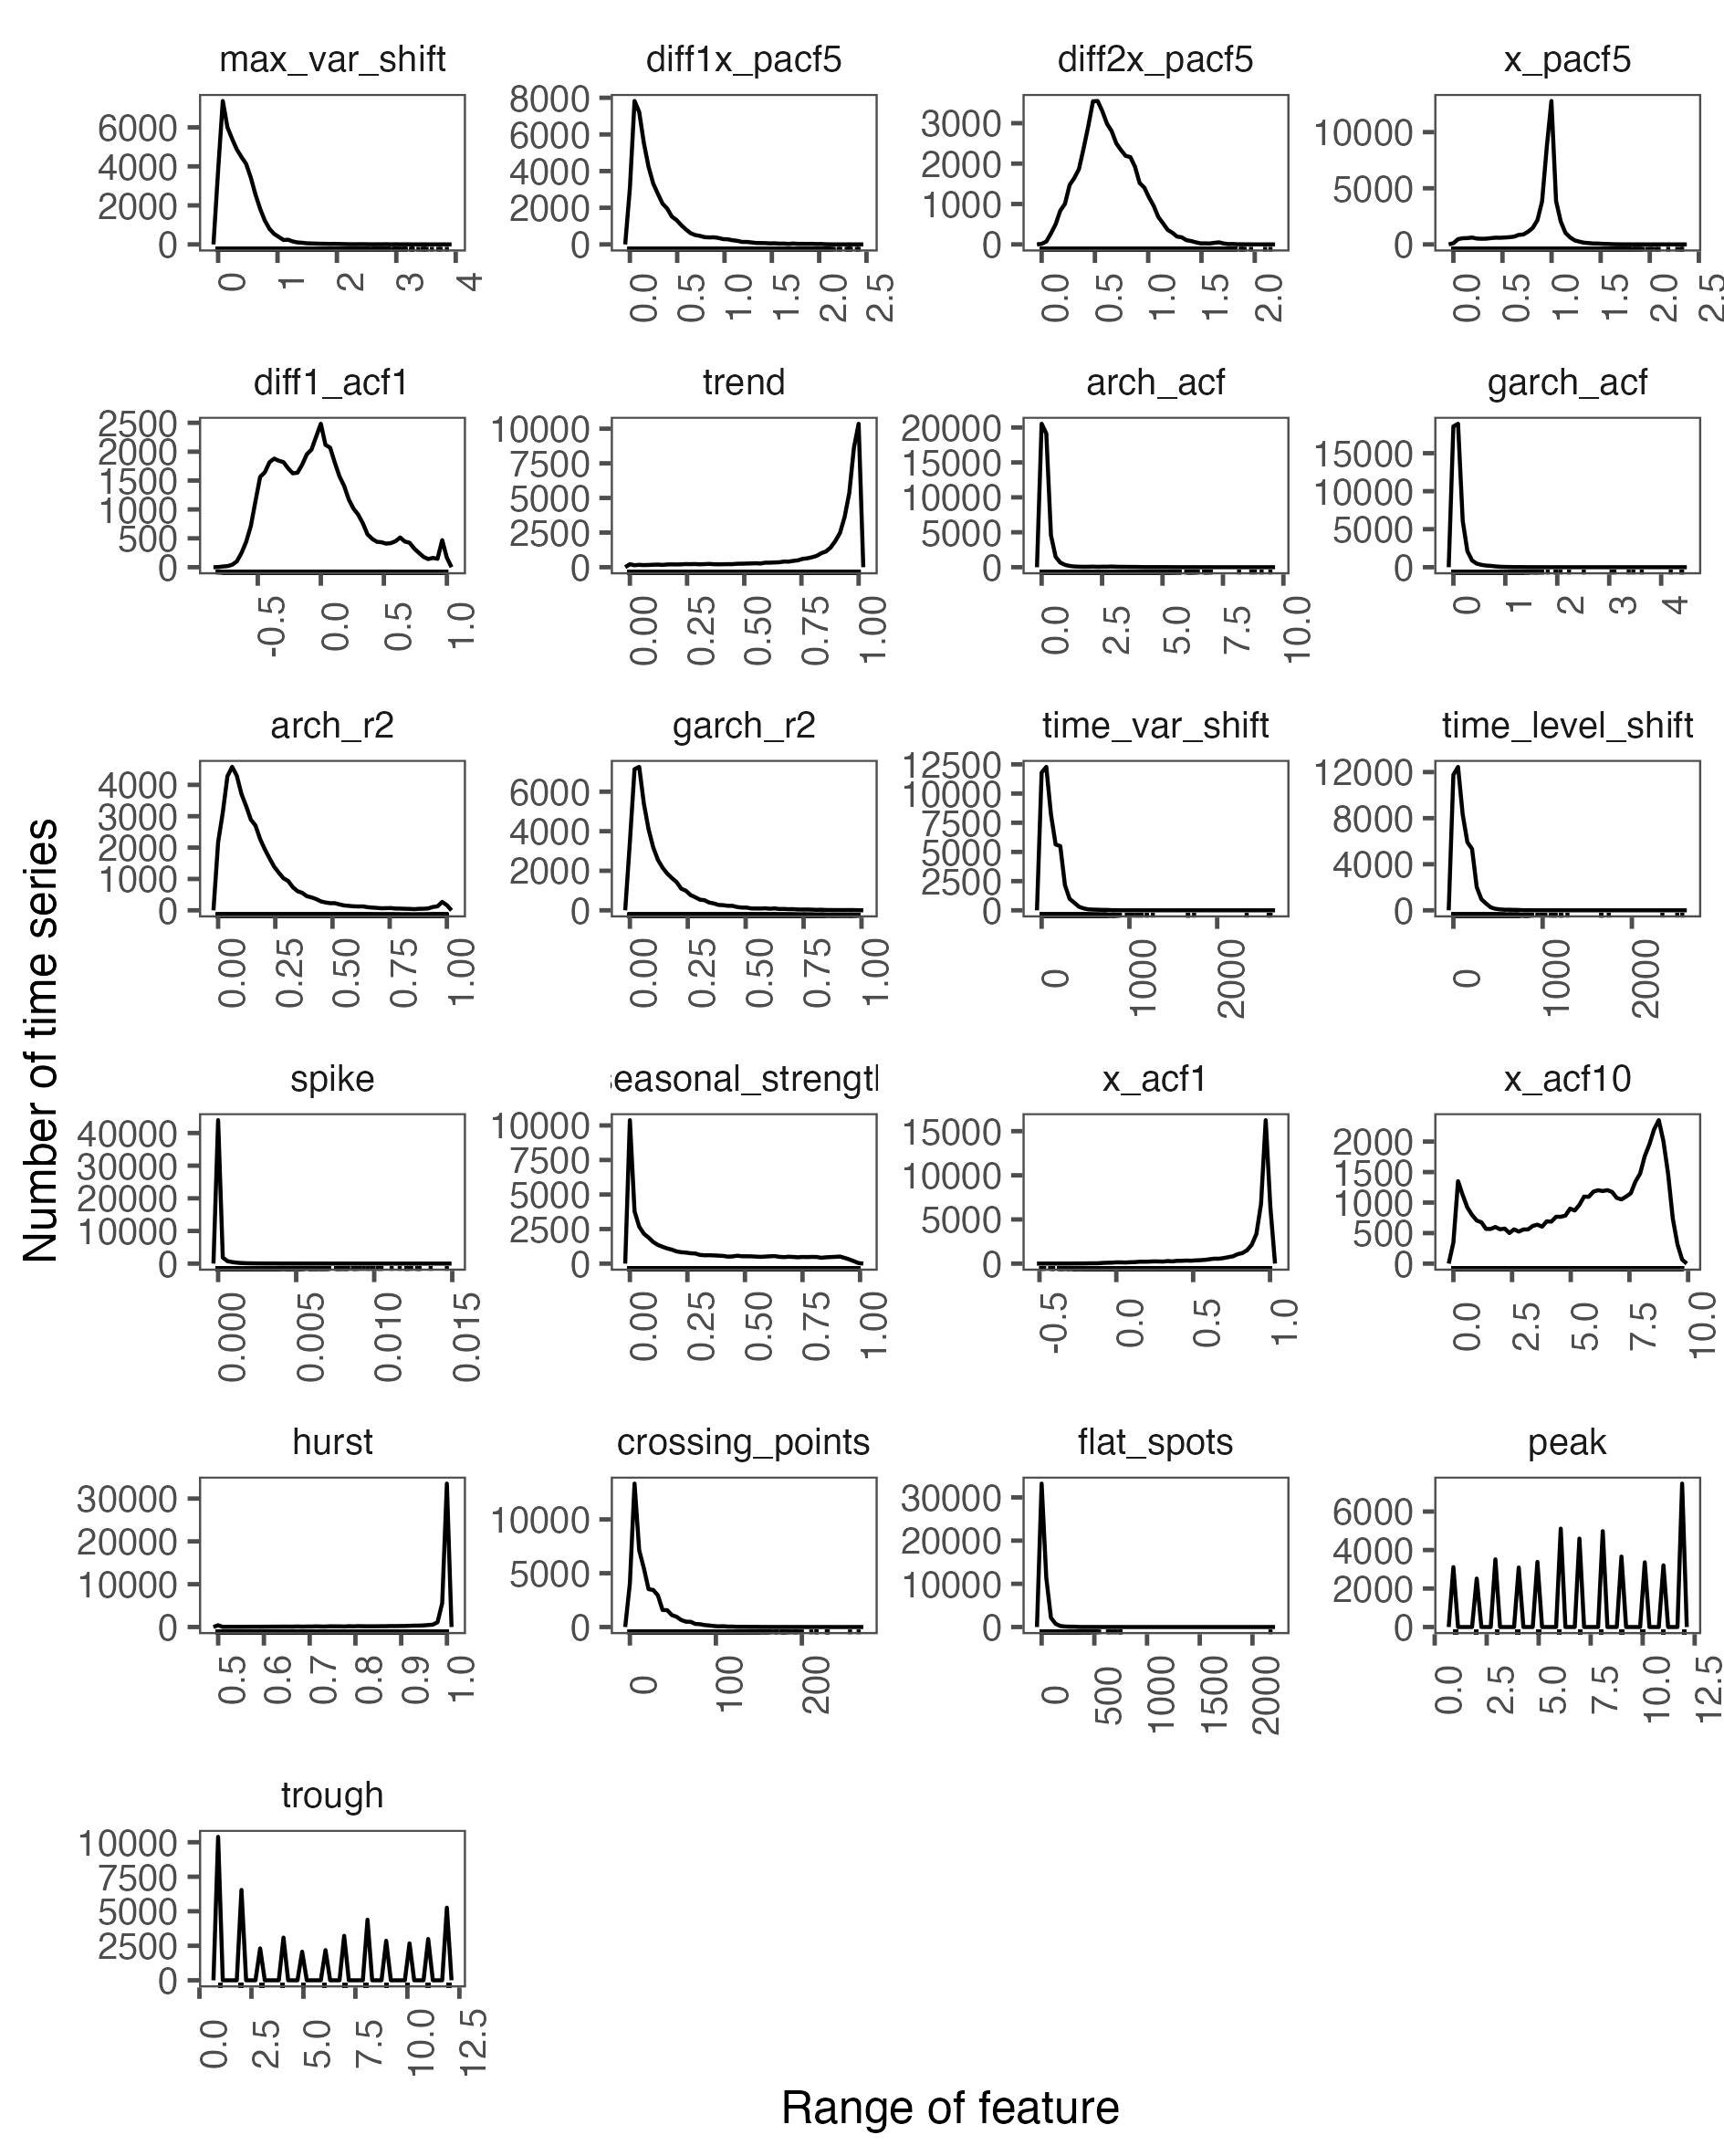
\includegraphics[width=0.7\linewidth]{img/300dpi/featurets_selection2} 

}

\caption{   extcolor{blue}{Features of monthly time series from M4 competition dataset (continue)} }\label{fig:feature2}
\end{figure}

\hypertarget{taeffect}{%
\subsection{Effect of temporal aggregation on time series
features}\label{taeffect}}

In addition to \textcolor{blue}{extract the features} of monthly time
series, we also compute features after transforming the time series to
bi-monthly, quarterly, 4-monthly, semi-annual and annual granularity. We
use these features to demonstrate how non-overlapping temporal
aggregation may change time series features. To highlight the effect of
NOTA, we first started by plotting the distribution of features at each
level, however the difference between distributions was not revealing
because features have log-tail distributions. Instead, we categorise
features of the original series to into four categories using quantiles:

\begin{itemize}
\tightlist
\item
  If \(0 < feature \leqslant 0.25\), Category = Very low
\item
  If \(0.25 < feature \leqslant 0.5\), Category = Very low
\item
  If \(0.5 < feature \leqslant 0.75\), Category = Very low
\item
  If \(0.75 < feature \leqslant 1\), Category = Very low
\end{itemize}

We then calculate the mean of features for each category and each time
granularity. The results have been illustrated in Figure
\ref{fig:featureagg1} and \ref{fig:featureagg2}. They show how time
series features change from monthly to annual granularity for the time
series features. The results indicate that as the level of time
granularity increases from monthly to annual, some features become
weaker and may disappear, while others dominate the series.

\begin{figure}[H]

{\centering 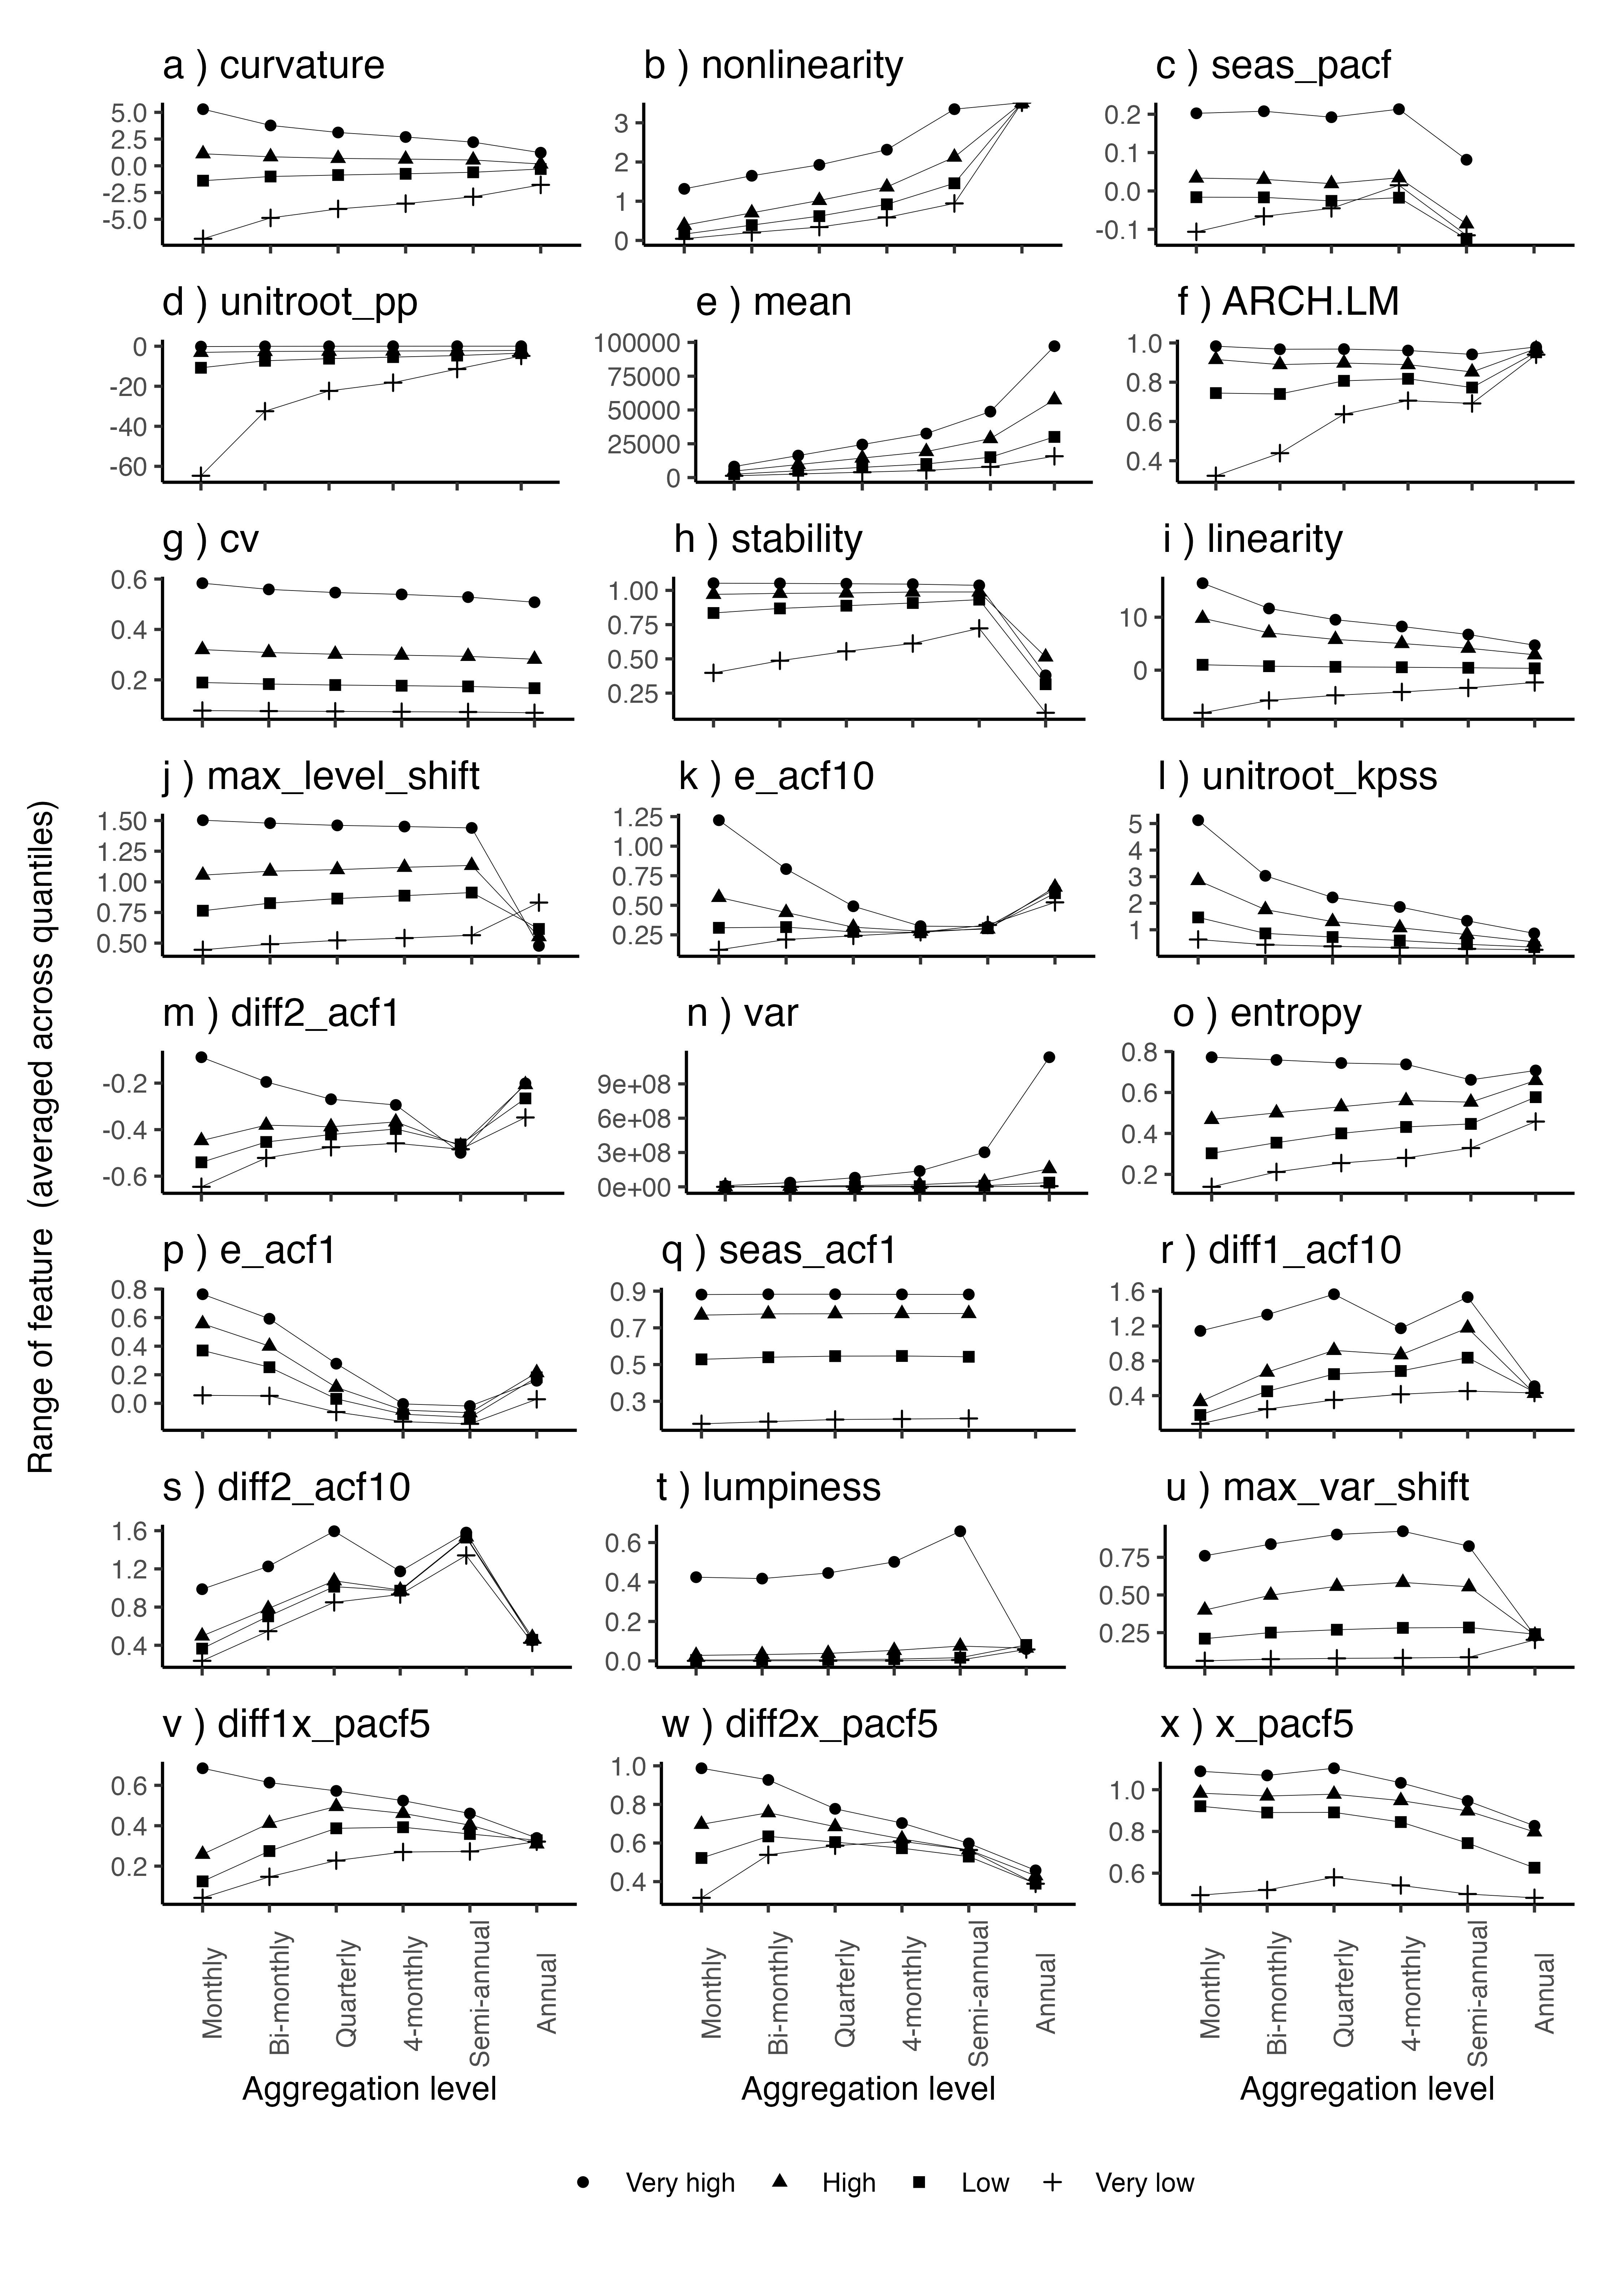
\includegraphics[width=0.7\linewidth]{img/mp_category_all1} 

}

\caption{   extcolor{blue}{The effect of non-overlapping temporal aggregation on monthly time series features of M4 competition dataset} }\label{fig:featureagg1}
\end{figure}

We observe a decrease in curvature as we aggregate and it approaches
zero at annual level, while nonlinearity increases with aggregation
indicating that series become more non-linear. Mean increases and
variance decreases, however the effect is higher for very high category.
We also observe that coefficient of variation decreases. Linearity is
pushed toward zero if it is high or low, meaning that series at annual
level losses its linearity feature. Both uniroot\_pp and unitroot\_kpss
become close to zero with increasing aggregation level, highlighting the
fact that series become more non-stationary if the monthly series
\textcolor{blue}{is stationary}, otherwise it \textcolor{blue}{remains}
almost the same. The measures related to seasonality such as seasonal
strength, autocorrelation lag1 and the sum of squared of the first 10
autocorrelation decreases. It is interesting to observe that entropy
increases with aggregation if it is not very high at monthly level,
meaning that series become difficult to forecast. However we see a
reduction in entropy if it is very high at the monthly level. We also
observe an increase for ARCH.HM especially if it is very low at the
monthly level. If it is very close to one, it stays almost unchanged.

\begin{figure}[H]

{\centering 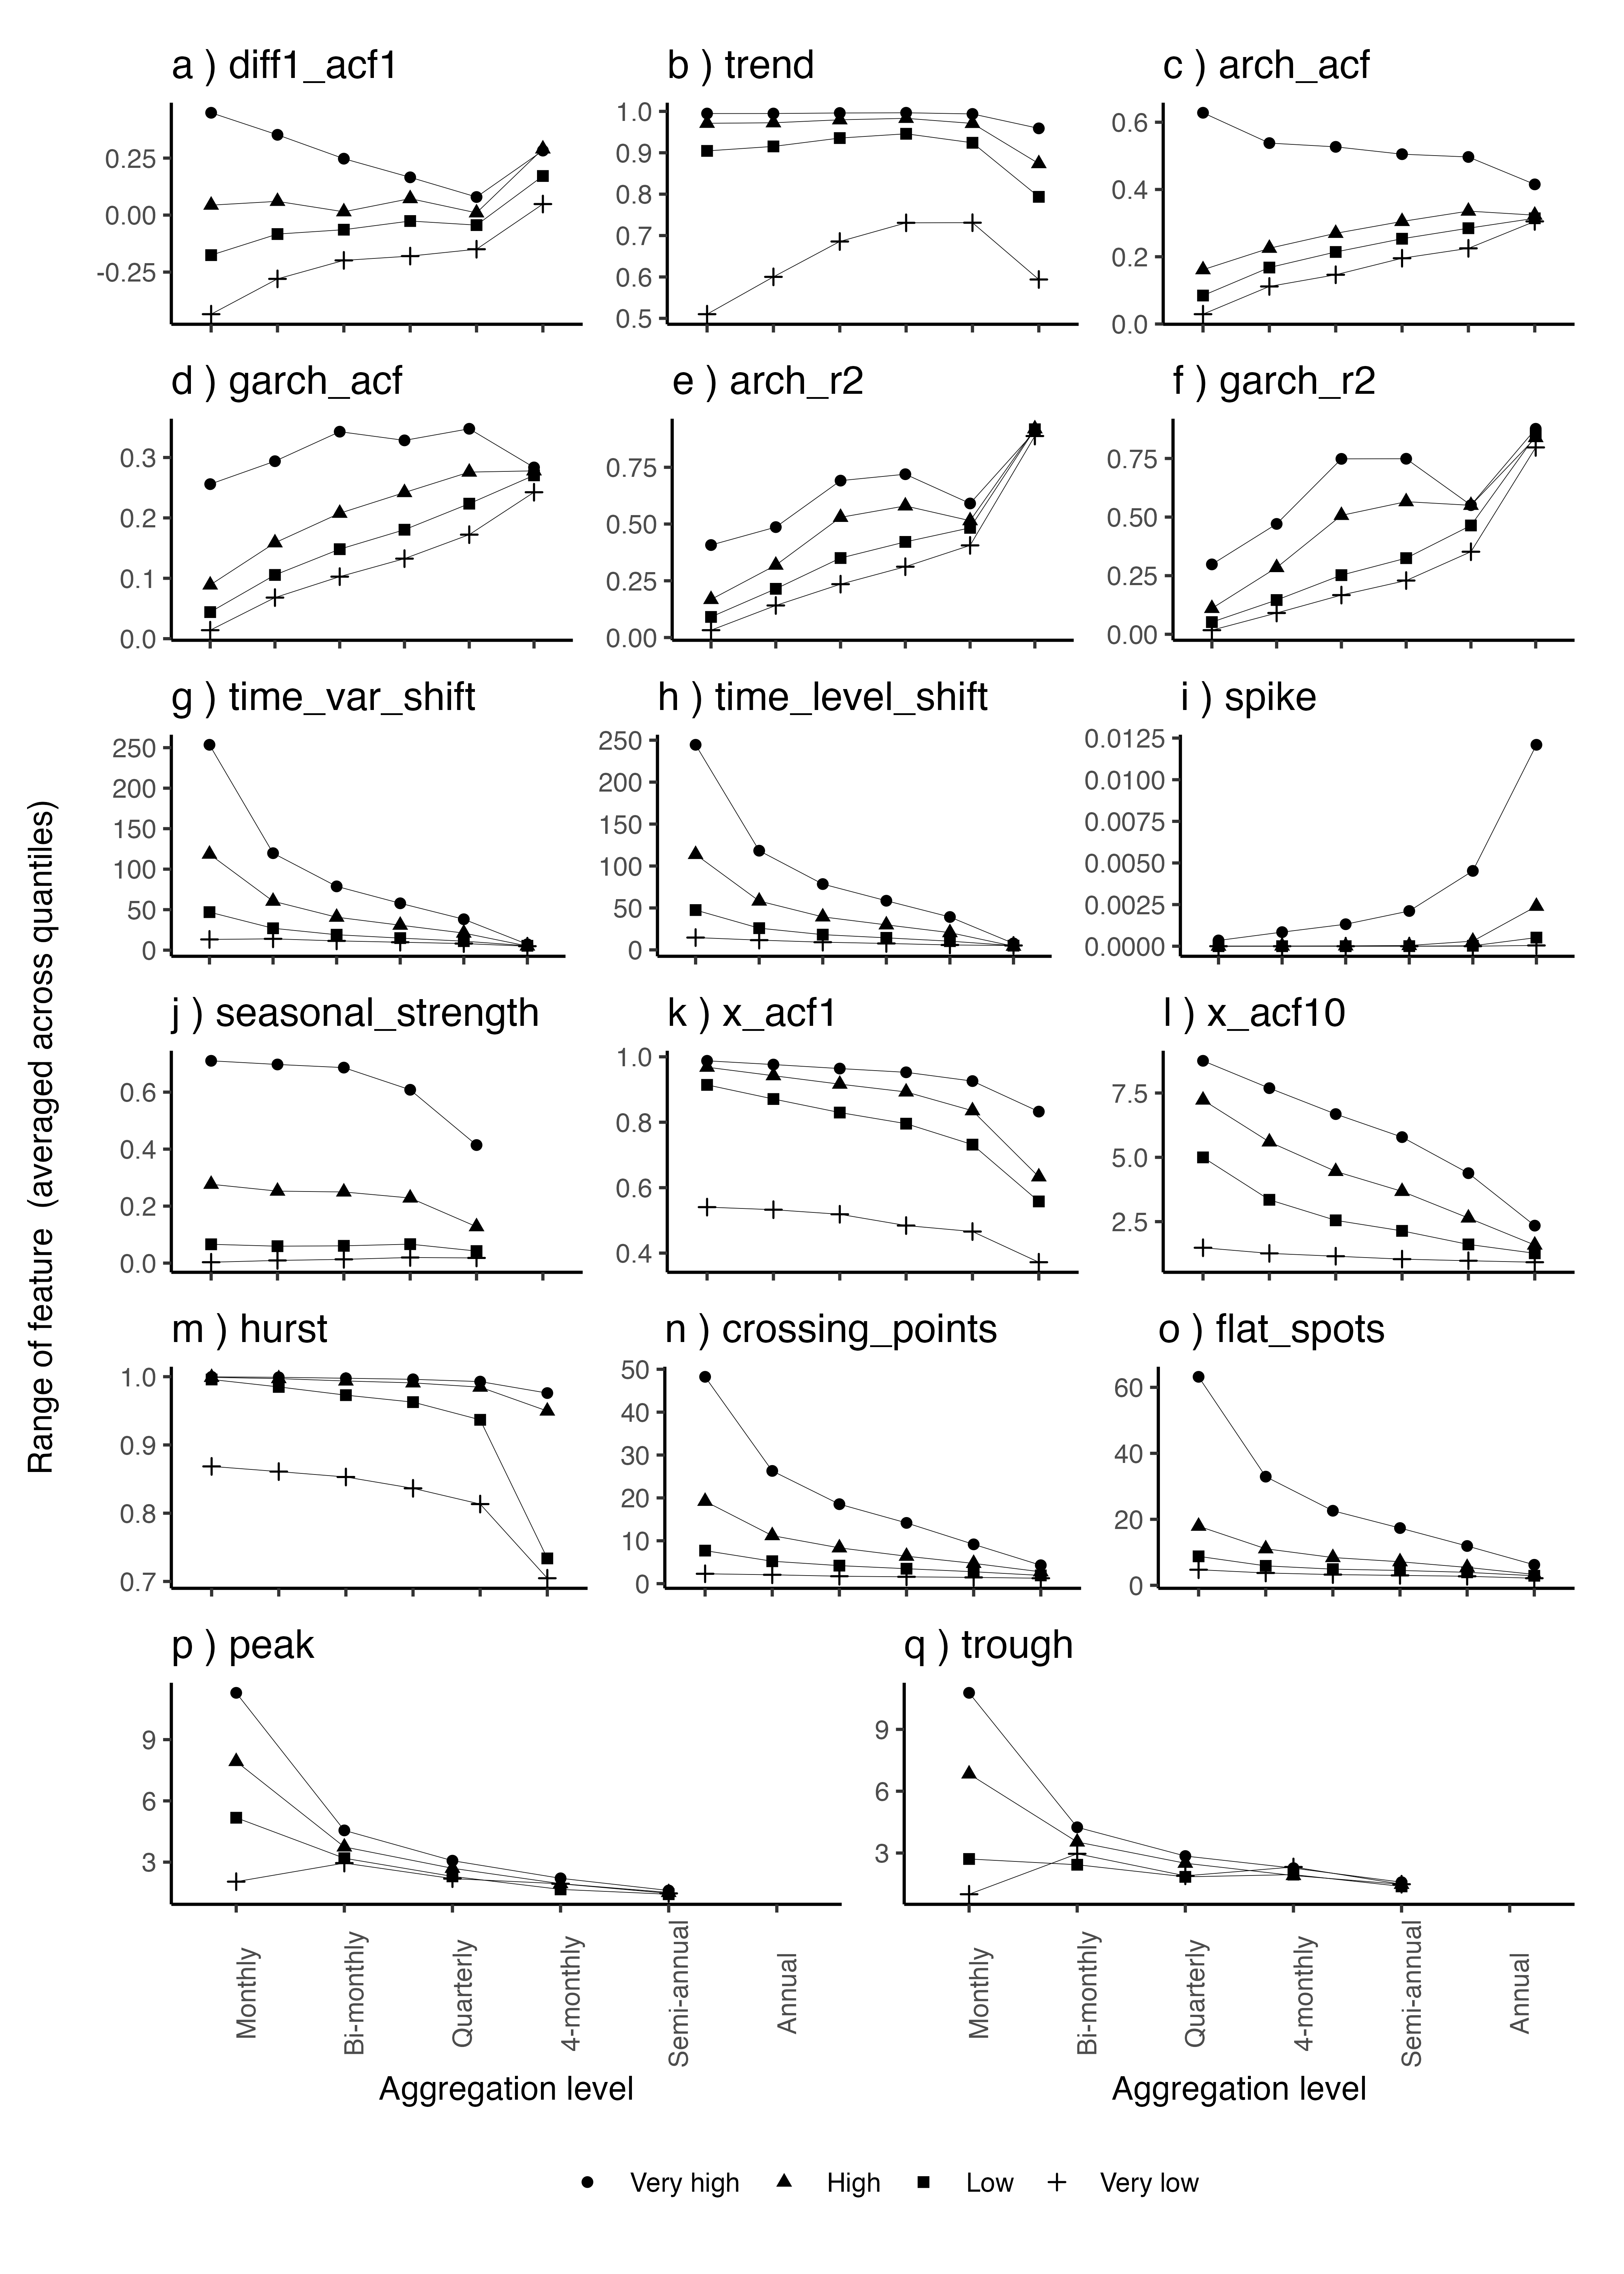
\includegraphics[width=0.7\linewidth]{img/mp_category_all2} 

}

\caption{   extcolor{blue}{The effect of non-overlapping temporal aggregation on monthly time series features of M4 competition dataset (continue)} }\label{fig:featureagg2}
\end{figure}

We should note that some features are not stable and show chaotic
behaviors at the annual level. This might be because these features are
not measurable for some time series. Therefore, they are returned as NA
(not known) and are removed when calculating the mean of each category,
hence the disorder of these features at the annual level.

\hypertarget{forecast-accuracy-evaluation-of-ad-and-af-approaches}{%
\subsection{Forecast accuracy evaluation of AD and AF
approaches}\label{forecast-accuracy-evaluation-of-ad-and-af-approaches}}

In this study, we aim at generating forecasts for a forecast horizon
aggregation, lead-time period, using AF and AD approaches. While the
original time series granularity is monthly, we require forecasts to be
produced at Bi-monthly (aggregation level = 2), Quarterly (aggregation
level = 3), 4-monthly (aggregation level = 4), Semi-annual (aggregation
level = 6) and annual (aggregation level = 12).

Figure \ref{fig:RMSSE} displays a boxplot of RMSSE measure created for
all 48,000 series at various level of forecast granularities. Results
demonstrate that both AF and AD approaches might outperform each other
for different time series. However, AF approach is generating
consistently more accurate forecasts through all aggregation levels and
the difference becomes more pronounced as aggregation level increases.
The difference is especially notable at the annual level. From 48000
monthly time series, the AF approach was superior in 30,147 cases
(\(63\%\)) compared to 17,853 cases (\(37\%\)) for AD when forecasting
annual time granularity.
\textcolor{blue}{These results might be surprising, because common recommendation based on practice and in the literature (see Section \@ref{lit}) is to use AD over AF.}
However, we should note that almost all these studies report the overall
accuracy improvement rather than the forecast accuracy at the series
level. Our results show that recommending AD to forecast over the
forecast horizon aggregation/lead-time might not necessarily lead to
more accurate forecast. Moreover, AF is shown to be a very competitive
forecasting strategy. This might be due to the time series features of
the monthly time series discussed in section \ref{mtsmeasure}.

\begin{figure}[H]

{\centering 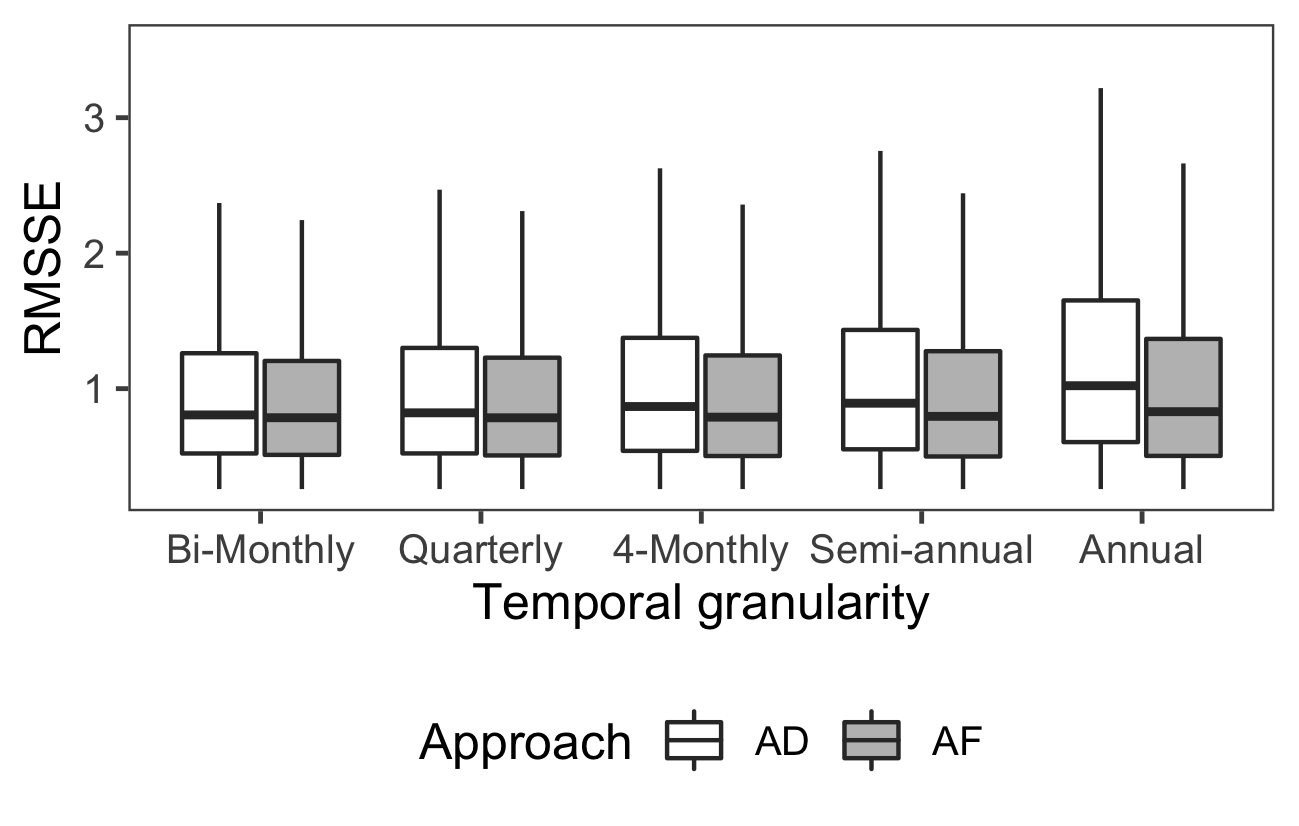
\includegraphics[width=0.7\linewidth]{img/300dpi/box_plot_rmsse} 

}

\caption{RMSSE errors through aggregation levels.}\label{fig:RMSSE}
\end{figure}

We have also conducted a statistical test using MCB (Multiple Comparison
with the Best method) \citep{MCB} to assess the statistical significance
in the performance of AF and AD approaches.

From Figure \ref{fig:MCB}, it is evident that there is a statistical
difference between forecasts generated from AF and AD. The forecasts
generated from AD approach are less accurate, while the strategy of
aggregating forecasts proves to be more accurate. The results were
cross-validated through multiple forecast horizons (h=12, 24 and 60) and
via several other error metrics as described in \ref{errormetric}. The
main conclusions are almost perfectly aligned with results demonstrated
in Figure \ref{fig:MCB}.

\begin{figure}[H]

{\centering 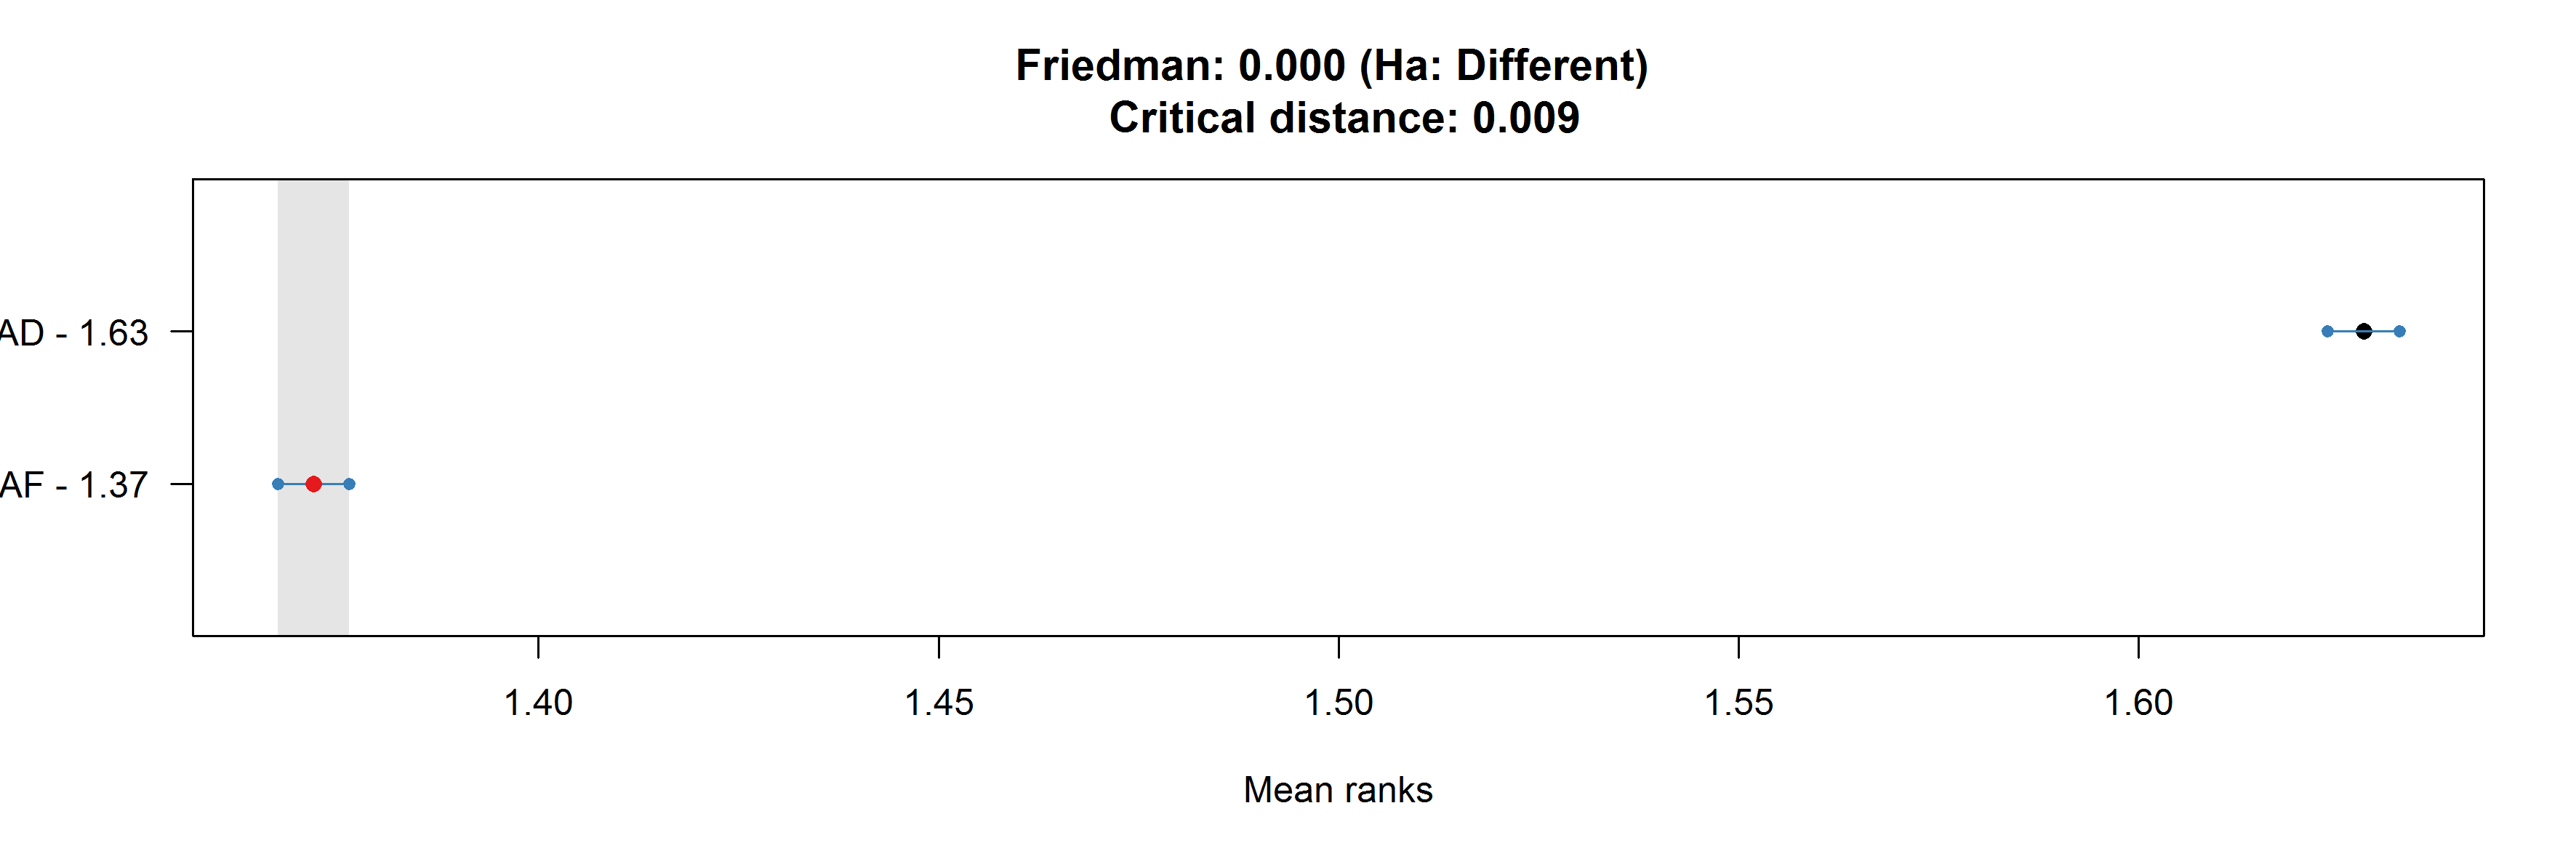
\includegraphics[width=1\linewidth]{img/300dpi/Fig_MCB} 

}

\caption{   extcolor{blue}{Performance of AF and AD models evaluated through MCB test. RMSSE values are used for computing the ranks and a 95 percentile confidence level.}}\label{fig:MCB}
\end{figure}

In Figure \ref{fig:RMSSE}, we showed that both AF and AD have diverging
performance through different levels of aggregation. Moreover, Figure
\ref{fig:featureagg1} and \ref{fig:featureagg2} demonstrate the
evolution of the time series features through these levels. We believe
that the presence of certain time series features might favorite AD or
AF. We should note that the results presented for the rest of the paper
are based on forecasts produced for the annual level (aggregation level
= 12) using AF and AD approaches. This is because we see the highest
difference in the performance at the annual level, and when the time
series granularity is monthly, very often forecast is required at the
annual level.

In the next section, we build machine learning models to explore the
association between time series features and the forecasting performance
of AF and AD performance.

\hypertarget{ml}{%
\section{Machine learining models}\label{ml}}

In this section, we use several models to shed lights on the association
between time series features and the performance of these approaches.
Using the time series features extracted at monthly time granularity and
the RMSSE error metric generated for each approach (i.e.~AF and AD), we
build machine learning algorithms to reveal relevant sets of features
affecting the performance of these approaches. The first step in
building such a model is to construct a dataset consisting of time
series features and model class labels for a given time series.
Therefore, we turn this problem into a classification supervised
learning, using features as predictors and the winning approach labeled
as AD or AF as the response variable or the outcome for each time
series. We discover, extract and present the details on which time
series features are the most influential on the accuracy of AF and AD
approaches. In addition to interpretability, the algorithm should be
able to accurately predict which model to use with a given set of time
series features in the original series. We have used the RMSSE at the
annual level given the pronounced difference in accuracy at that level.

Figure \ref{fig:featuresmatrix} shows a grid of scatterplots showing the
bivariate interactions between various pairs of features. Each point
corresponds to one time series. The figure also highlights the winning
approach (i.e.~either AF or AD) when forecasting for annual time
granularity. The black dots represent the situations where AD was more
accurate, while yellow dots represent the opposite. Given the number of
features used in this study, it is unfeasible to include the scatterplot
matrix for all pairs of features. Figure \ref{fig:featuresmatrix} shows
only the pairs plot for 10 features.

\begin{figure}[H]

{\centering 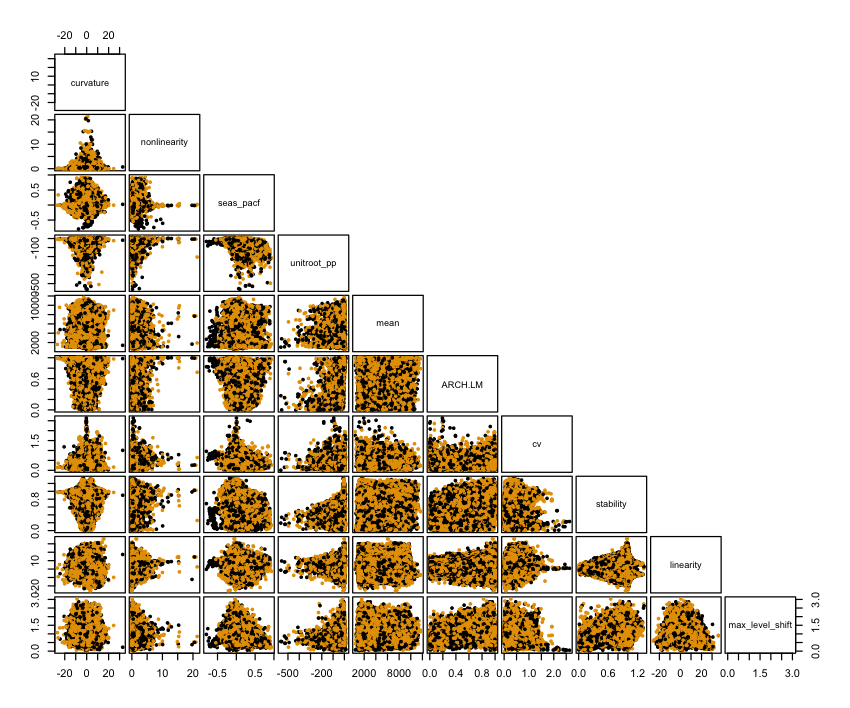
\includegraphics[width=1\linewidth]{img/300dpi/pair_plot} 

}

\caption{Time series features matrix. Each point indicates one single time series with a feature in x-axis and another at y-axis. The black and yellow colors show the outperformance of AD and AF, respectively.}\label{fig:featuresmatrix}
\end{figure}

Figure \ref{fig:featuresmatrix} demonstrates a perplexed relationship
between features and AD/AF approaches, with a lot of noise, confounding
features and lack of clear decision boundaries between AD and AF
performance. It is clear that some features might have linear or
non-linear relationships with each other, while others might be
unrelated. For most of features presented in Figure
\ref{fig:featuresmatrix}, there is no strong relationship.

Considering the complicated boundaries and relationship between
predictors, we develop several machine learning algorithms to discover
patterns and connections between time series features and the accuracy
of the AF and AD approaches.

\hypertarget{evaluating-the-prediction-accuracy-fo-models-in-classification}{%
\subsection{Evaluating the prediction accuracy fo models in
classification}\label{evaluating-the-prediction-accuracy-fo-models-in-classification}}

In this section, we examine the prediction accuracy of the ML models in
classifying whether AD or AF should be used to forecast the horizon
aggregation of a given time series, based on its features. We report the
prediction accuracy of the ML classifiers using measures discussed in
section \ref{errormetric}. We have designed an interactive ShinyApp that
includes the prediction accuracy of ML approaches and can be accessed by
readers \footnote{https://supplychainanalytics.shinyapps.io/Evaluation\_of\_ML\_models/.}.

Table \ref{tab:cost} demonstrates that RF model has the best performance
with the lowest misclassification error, highest F statistics and one of
the best AUC statistics.

\begin{table}
\caption{\label{tab:cost}Comparison of different ML models}
\centering
\begin{tabular}[t]{lccc}
\hline
 & F-statistics & Misclassification error & AUC\\
\hline
LR &  0.6083881 &  0.4383333 & 0.5676151\\
\hline
LDA & 0.7655532 & 0.3718750 & 0.5130521\\
\hline
QDA &  0.7121420 & 0.3929861 & 0.5499207\\
\hline
KNN &  0.6882851 & 0.3911806 & 0.5814969\\
\hline
Lasso & 0.6368112 & 0.4252083 & 0.5677939\\
\hline
GAM &  0.6042137 & 0.4383333 & 0.5707890\\
\hline
RF & 0.7773134 & 0.3367361 & 0.5704724\\
\hline
Boosting & 0.7646663 & 0.3640972 & 0.5267067\\
\hline
SVM & 0.7646663 & 0.3640972 & 0.5318491\\
\hline
DTW & 0.7093325 & 0.3888889 & 0.5616327\\
\hline
FNN & 0.7649972 & 0.3724306 & 0.5128323\\
\hline
DL Torch & 0.7649434 & 0.3678472 & 0.5230656\\
\hline
XG Boost & 0.7688268 & 0.3423611 & 0.5728495\\
\hline
TensorFlow & 0.7669575 & 0.3690972 & 0.5166527\\
\hline
RNN & 0.7659351 & 0.3710417 & 0.5142032\\
\hline
CNN & 0.7662412 & 0.3700694 & 0.5158014\\
\hline
\end{tabular}
\end{table}

\begin{figure}[H]

{\centering 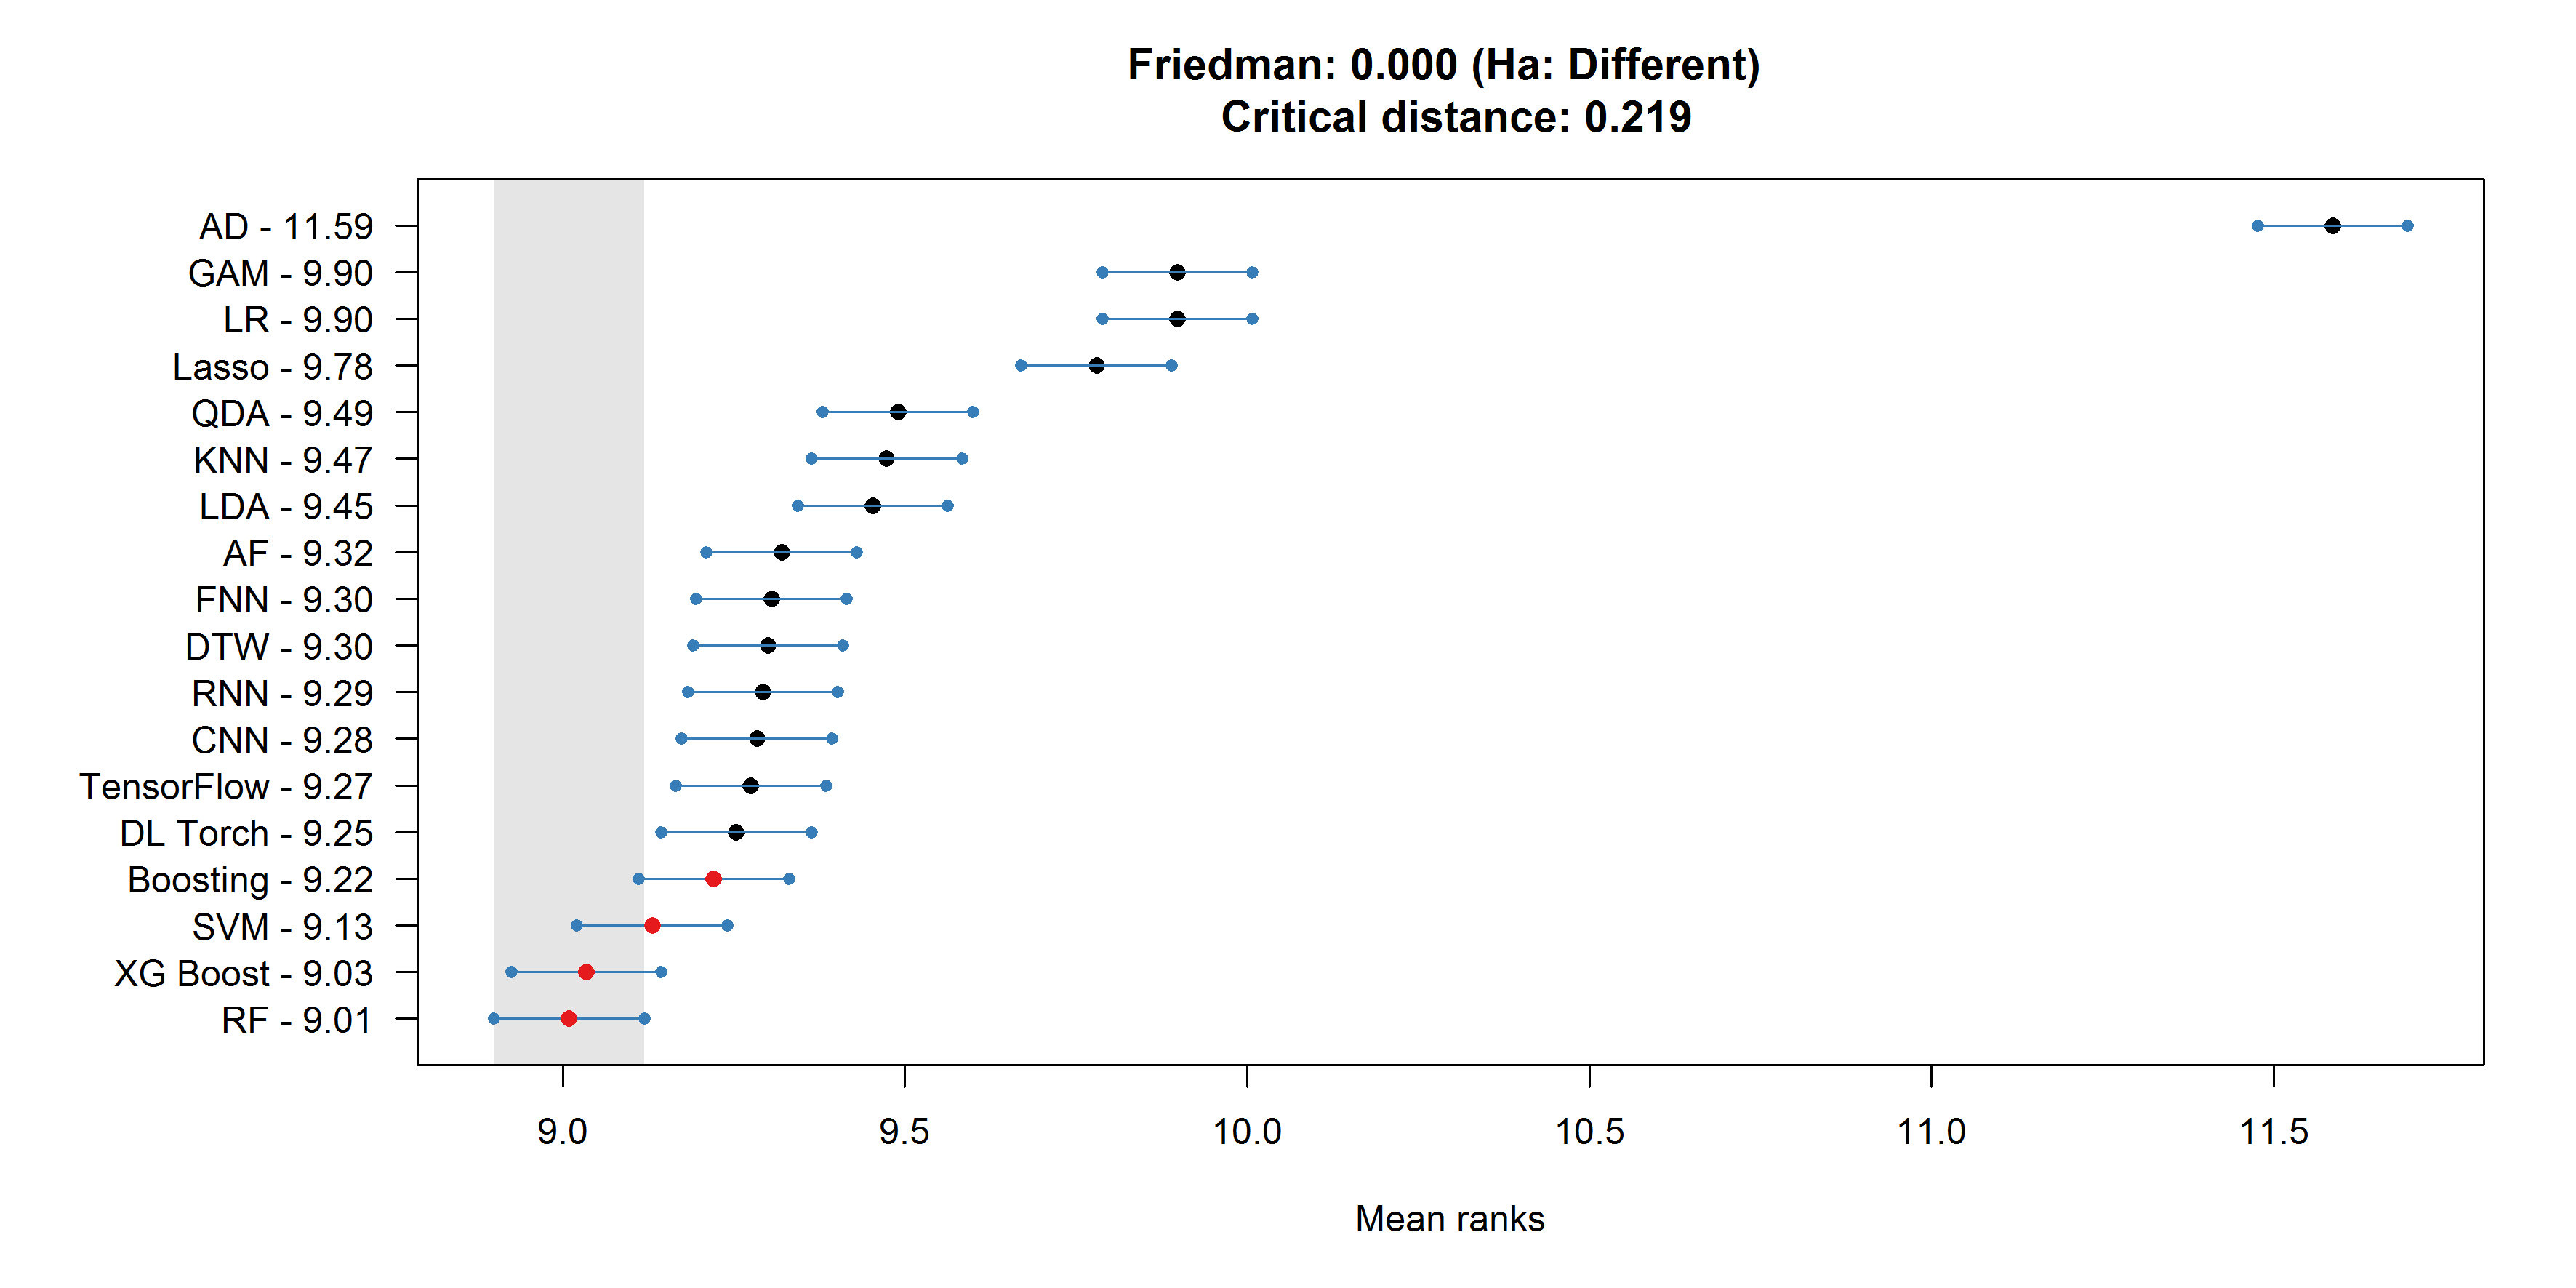
\includegraphics[width=1\linewidth]{img/300dpi/Fig_MCB_all(review)} 

}

\caption{\textcolor{blue}{Performance of different models evaluated through MCB test. RMSSE errors are used for computing the ranks and a 95 percentile confidence level.}}\label{fig:MCB_ML}
\end{figure}

The Figure \ref{fig:MCB_ML} shows the result of MCB test conducted to
examine the difference between the performance of ML algorithms. The
results show that there is a statistically significant difference
between the performance of RF and all other models. According to the MCB
test, AD approach generated the most inaccurate forecasts and therefore
drastically underperformed compared to the others. All other ML models
have much better performance, and the RF comes out as the ultimate
winner in terms of mean rank classification accuracy on the test data
set.

We also perform the utility evaluation of ML models. The results are
presented in the Table \ref{tab:matrix}. The Table \ref{tab:matrix}
represents the average values of RMSSE for AD and AF approaches when the
correct classification was AD and AF, respectively. When the true model
to use is AD (17,853 causes), the average RMSSE error is 0.9028 for AD,
and 1.5204 for AF. On the contrary, when the true model to use is AF
(30,147 causes), the average RMSSE error is 1.6568 for AD and 0.8669 for
AF. In this way, we design the average costs and benefits associated
with classification decisions and we are able to evaluate the ML models
performances via practical utility measure contribution connected to
their usage, and not just via standard statistical measures. This kind
of performance evaluation has much more value for practitioners
assessing the practical values of each ML model. The presented utility
evaluation can be further extended in practice by linking the monetary
costs to the decision based on the forecast. However, domain knowledge
on the area where forecasts are implemented is required.

\begin{table}
\caption{\label{tab:matrix}Cost and benefit matrix}
\centering
\begin{tabular}[t]{lccc}

\multicolumn{2}{c}{} & \multicolumn{2}{c}{\bf Actual}\\ 
\cline{3-4}
& & AD\  & AF\\
\hline
\multirow{2}{4em}{\bf Predicted} & AD & 0.902872 & 1.6568039\\
& AF & 1.520416 & 0.8669348\\
\hline
\end{tabular}
\end{table}

Figure \ref{fig:tableCB} demonstrates that RF has the smallest utility
metric (cumulative average RMSSE) while performing the classification
task on the test data set. We have also included the Ideal model, a
model that always predict correctly, to highlight the deviation of ML
approaches from this benchmark and to reveal the maximum possible margin
for reducing the overall cumulative RMSSE. Therefore, our result shows
that RF also provides the most accurate result for a given time series
examined by utility metric.

\begin{figure}[H]

{\centering 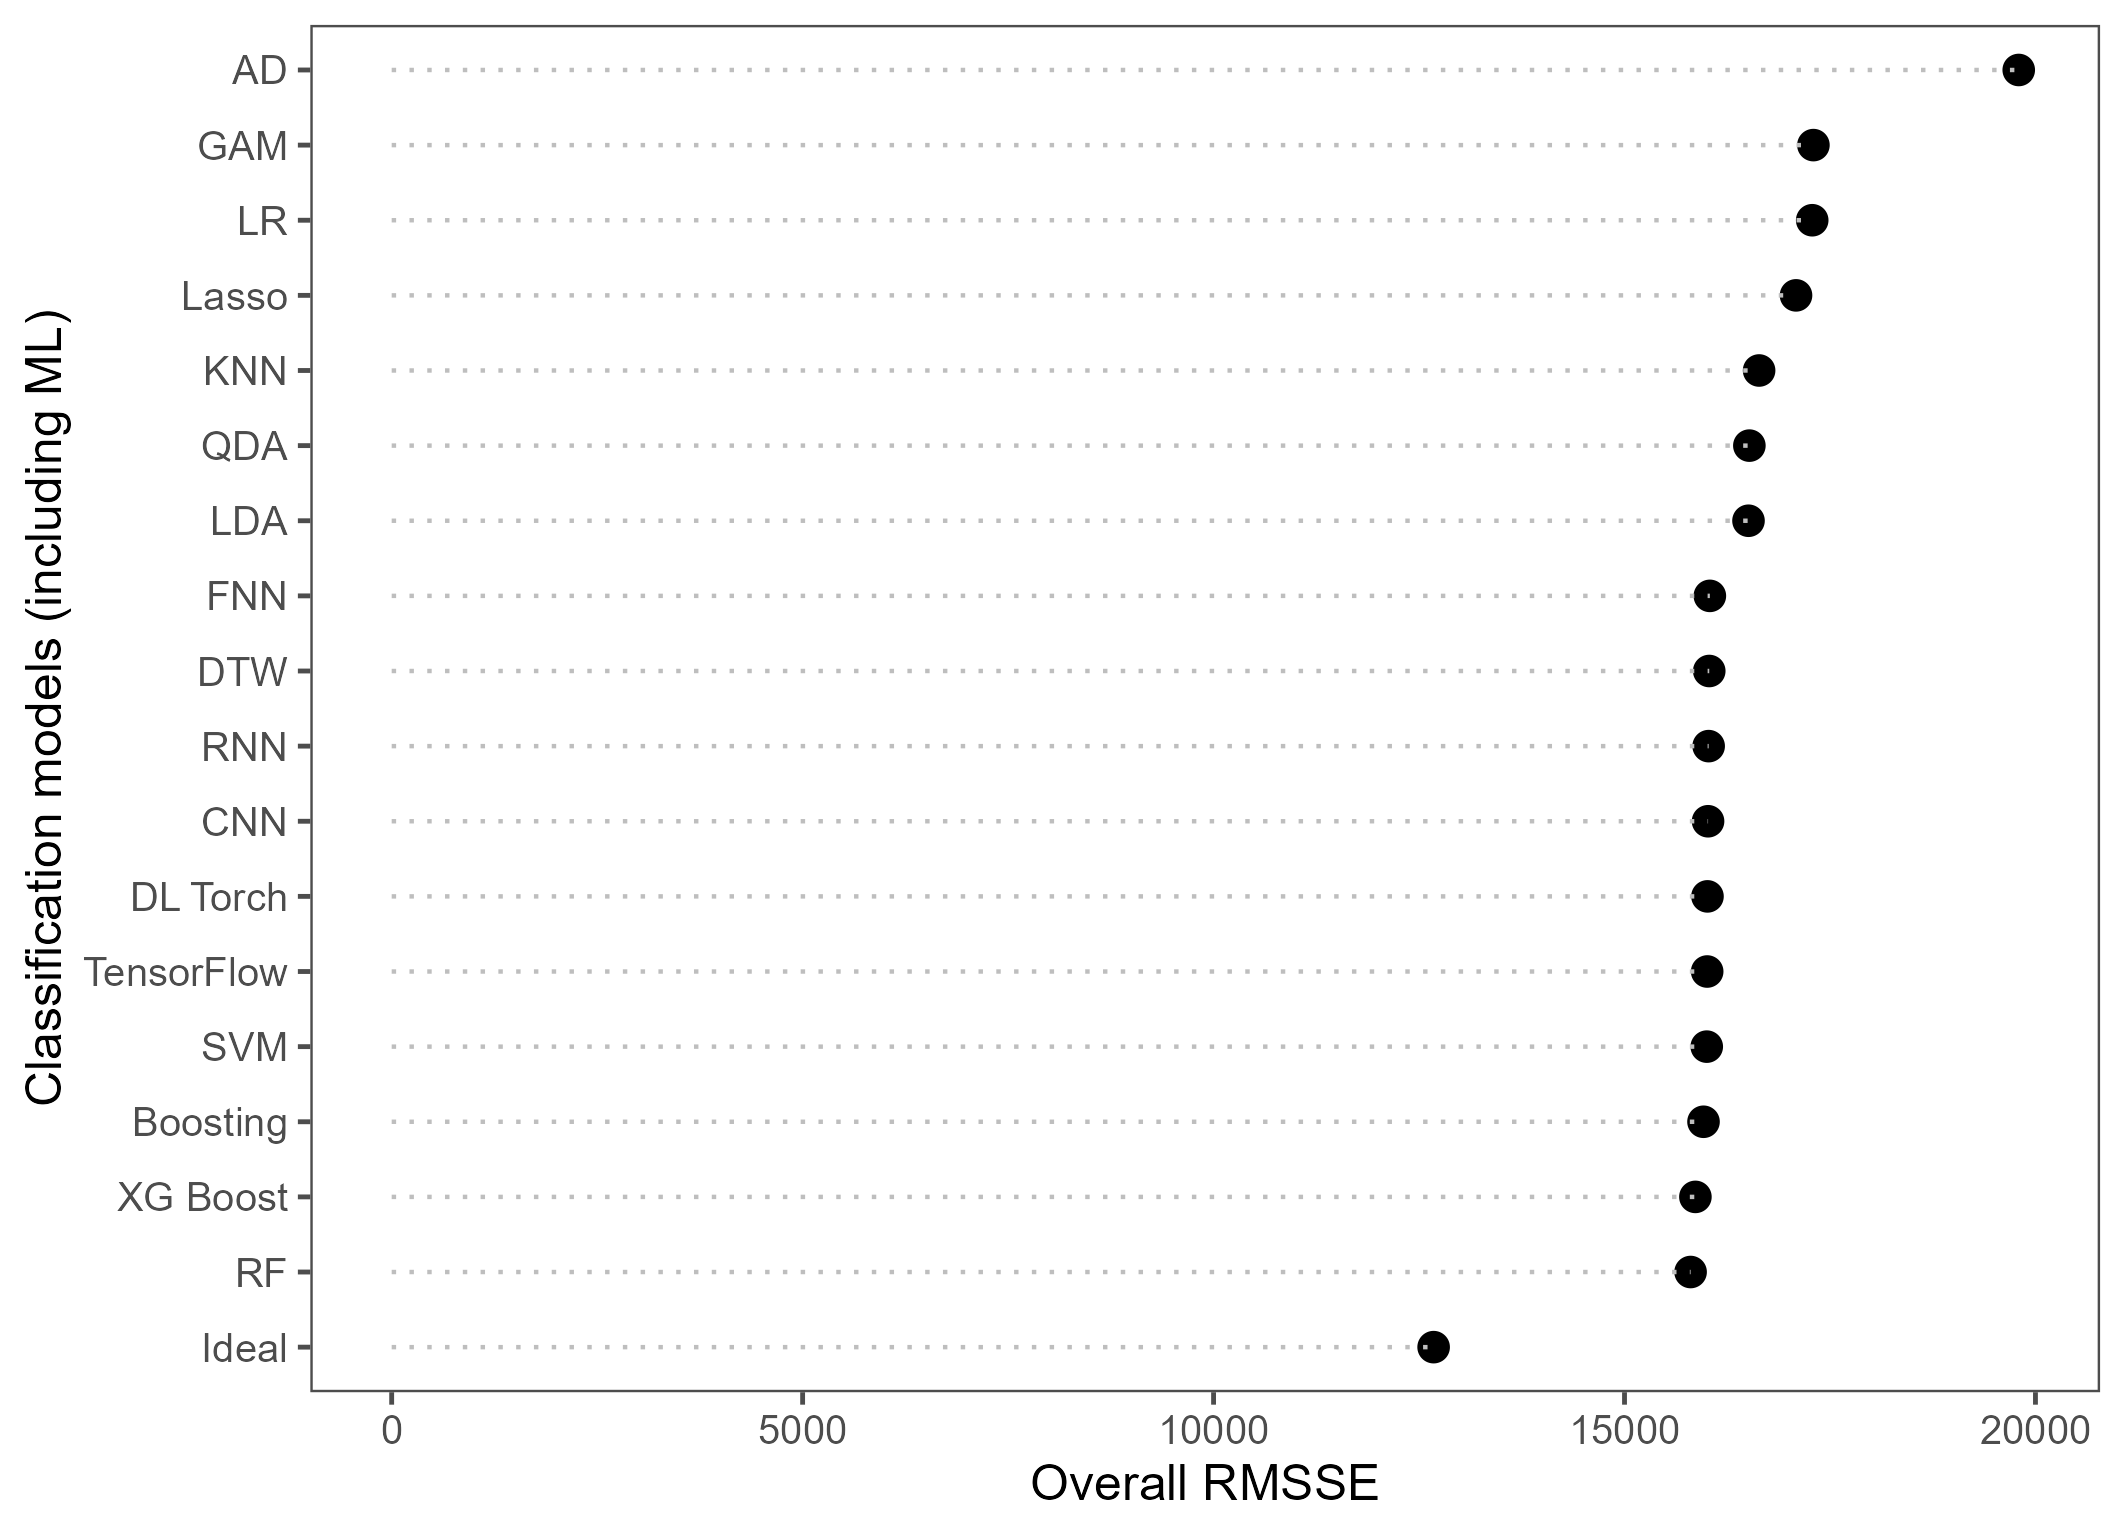
\includegraphics[width=0.6\linewidth]{img/300dpi/utility} 

}

\caption{Utility accuracy comparison}\label{fig:tableCB}
\end{figure}

\textcolor{blue}{We should note that we have conducted a comprehensive study and searched for optimal setups of each model rather than using automatic ML models. Additional information about the setup of models can be found in the Appendix or in the [GitHub repository](https://github.com/bahmanrostamitabar/time-searies-featute-temporal-aggregation).}

Among several algorithms, the RF provided the most accurate results
according to the several criteria. Therefore, we further discuss this
approach in the next section in more details.

\hypertarget{building-the-random-forest-algorithm}{%
\subsection{Building the random forest
algorithm}\label{building-the-random-forest-algorithm}}

Individually, these trees tend to overfit the data and generate future
forecasts with large variance. But, at the same time, they produce a low
bias. Therefore, in order to reduce the variance, the Bagging process is
building many trees on slightly different train data (since the data is
bootstraped-resampled) and averages forecasts of all the trees in one
unique forecast. For the sake of improving the Bagging process,
\citet{breiman2001random} introduced the RF as an algorithm that mimics
the Bagging process, but uses only a small random sample of the
available features, for building each classification tree. The idea
behind this is instead of just ``shaking'' the data via
bootstraped-resampled process, we are introducing additional randomness
in the process by ``shaking'' the features for the forecasting via
random sampling of just part of the features. Therefore, each time a
split in a tree is considered, a random sample of \emph{m} predictors is
chosen as a split candidates from the full set of \emph{p} features. A
fresh sample of \emph{m} features is taken at each split, and typically
\emph{m} \(\approx\) \(\sqrt p\) \citep{friedman2001elements}. By
forcing this process each time using the subsample of fresh features,
the RF is decorrelating each tree. In this way, the process of averaging
many different trees will reduce the variance more efficiently than in
the case of correlated trees.

In order to generate the RF model, there are several questions and
tuning parameters that need to be optimized so that the final model
could generate reliable and accurate forecasts. For that purpose,
\citet{friedman2001elements} have proposed the following methodology
presented in the Algorithm \ref{alg:RF}.

\begin{algorithm}
    \caption{Random Forest methodology.}
    \begin{algorithmic}[1]
      \item For {$b=1$ to $B$:}
        \begin{enumerate}[label=(\alph*)]
          \item Draw a bootstrap sample \textbf{Z*} of size $N$ from the training data.
          \item Grow a random forest tree $T_b$ to the bootstrapped data, by recursively repeating the following steps for each terminal node of the tree, until the minimum node size $n_{min}$ is reached.
            \begin{enumerate}[label=\roman*]
              \item Select $m$ variables at random from the $p$ variables.
              \item Pick the best variable/split-point among the $m$.
              \item Split the node into two daughter nodes.
            \end{enumerate}
       \end{enumerate}
  \item Output the ensemble of trees $\{T_b\}^B_1$.
    \end{algorithmic}
    \vspace{0.2cm}
    To make a prediction at a new point $x$:\\[0.2cm]
    \textit {Regression}: $\widehat{f}^B_{rf}(x)= \frac{1}{B} \sum_{b=1}^B T_b (x)$.\\[0.2cm]
    \textit {Classification}: Let $\widehat{C}_b(x)$ be the class prediction of the $b$th random-forest tree. \\ 
    \phantom{Classification } Then $\widehat{C}^B_{rf}(x)=majority\;vote\; \{{C}_b(x)\}^B_1$.
    \label{alg:RF}
\end{algorithm}

The first question is how many features to randomly choose for training
in each individual tree (i.e.~tree depth)? The question of how many
trees to use for fitting the RF model emerges, which also needs to be
answered in parallel. In order to determine the optimal number of
features and trees for building an RF model, the evaluation process is
performed with a different number of features and trees in each split.
Therefore, the resulting process represents the optimization problem of
seeking the minimum of the surface generated by features in each split,
trees and resulting out of the bag (OOB) forecasting error. (Please
refer to Figure \ref{fig:surface}). OOB represents the misclassification
error of the RF model while performing the classification tasks. Also,
OOB is the approximation of the cross validated test error, since the
process of fitting bootstrapped data sets consists of training the model
on just part of the original data and then predicting the remaining part
of the original data (i.e.~out of bag data). By averaging OOB errors
from many different tree models (which comprise the final random forest
model), the final OOB is obtained.

Figure \ref{fig:surface} reveals that increasing the number of trees
used for generating RF model reduces the misclassification error. A
similar scenario exists with features used in each split, where
increasing the number of features (up to a certain point) reduce
misclassification error. The presented surface is highly erratic and
undulating, making it hard to visually determine global minimum. For
that reason, the performance of the four best RF models with feature
splits (\emph{m} = 6, 10, 21 and 42) are shown through a different
number of trees used for fitting RF model (Figure \ref{fig:tree_depth}).

The Figure \ref{fig:tree_depth} represents the optimal number of splits
(randomly selected features) used during the process of building each
classification tree, according to OOB forecasting error. As demonstrated
in Figure \ref{fig:tree_depth} the OOB error is minimized on the depth
of 10. Therefore, the optimal number of features (i.e.~tree depth) for
the RF model is 10.

\begin{figure}[H]

{\centering 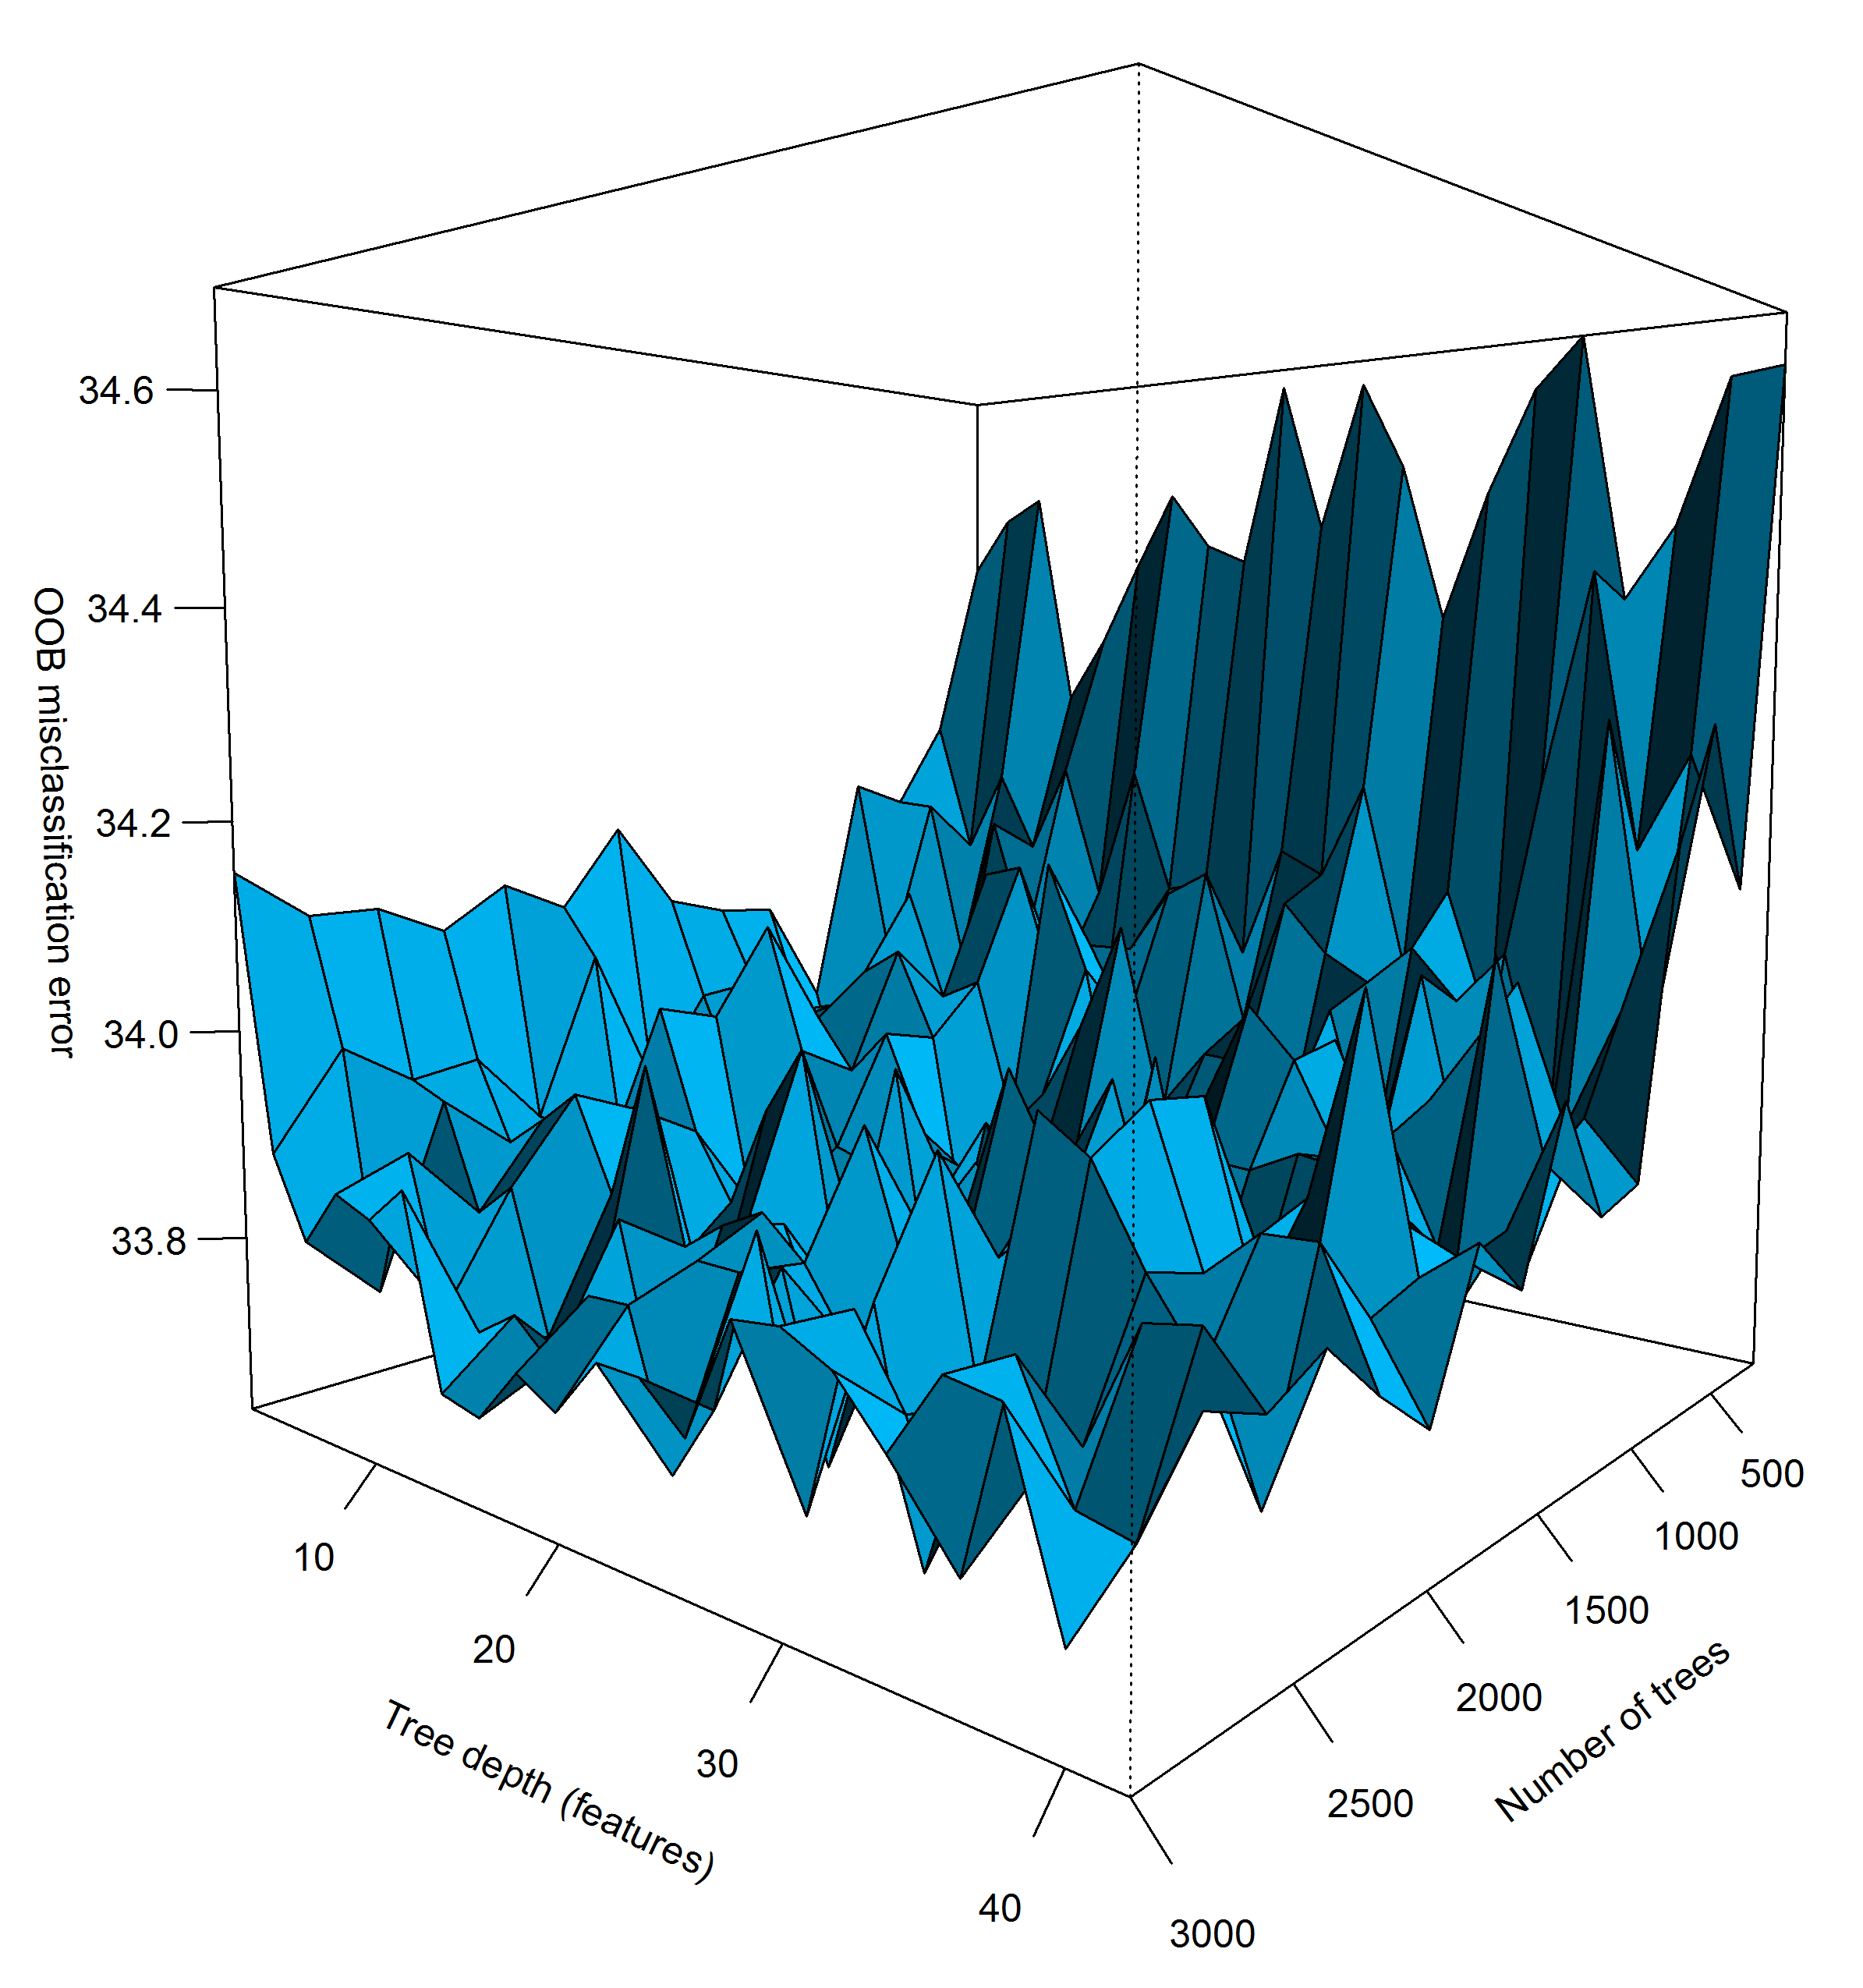
\includegraphics[width=0.7\linewidth]{img/300dpi/Fig_persp} 

}

\caption{Surface plot of the number of features (depth), number of trees and misclassification error of random forest model.}\label{fig:surface}
\end{figure}

The second tuning question is how many trees should be used for
generating the RF model? One of the good merits that help in this
process is the resilience of RF on overfitting
\citep{friedman2001elements}. Averaging process during the RF building
phase remedies the negative effects of choosing a large number of trees
for fitting the model, since this will not result in an increase in
variance on the test set. This implies that the penalty of choosing a
too large number of trees on models' overall performance is minor. The
criteria for this judgment is based on the OOB misclassification error,
which RF model produces on a given data set. Therefore, the optimal
number of trees is chosen by determining the number of trees where the
OOB misclassification error is stabilized (Figure \ref{fig:tree_depth}).
From Figure \ref{fig:tree_depth}, it is clear that error is stabilized
by using the 3000 trees.

\begin{figure}[H]

{\centering 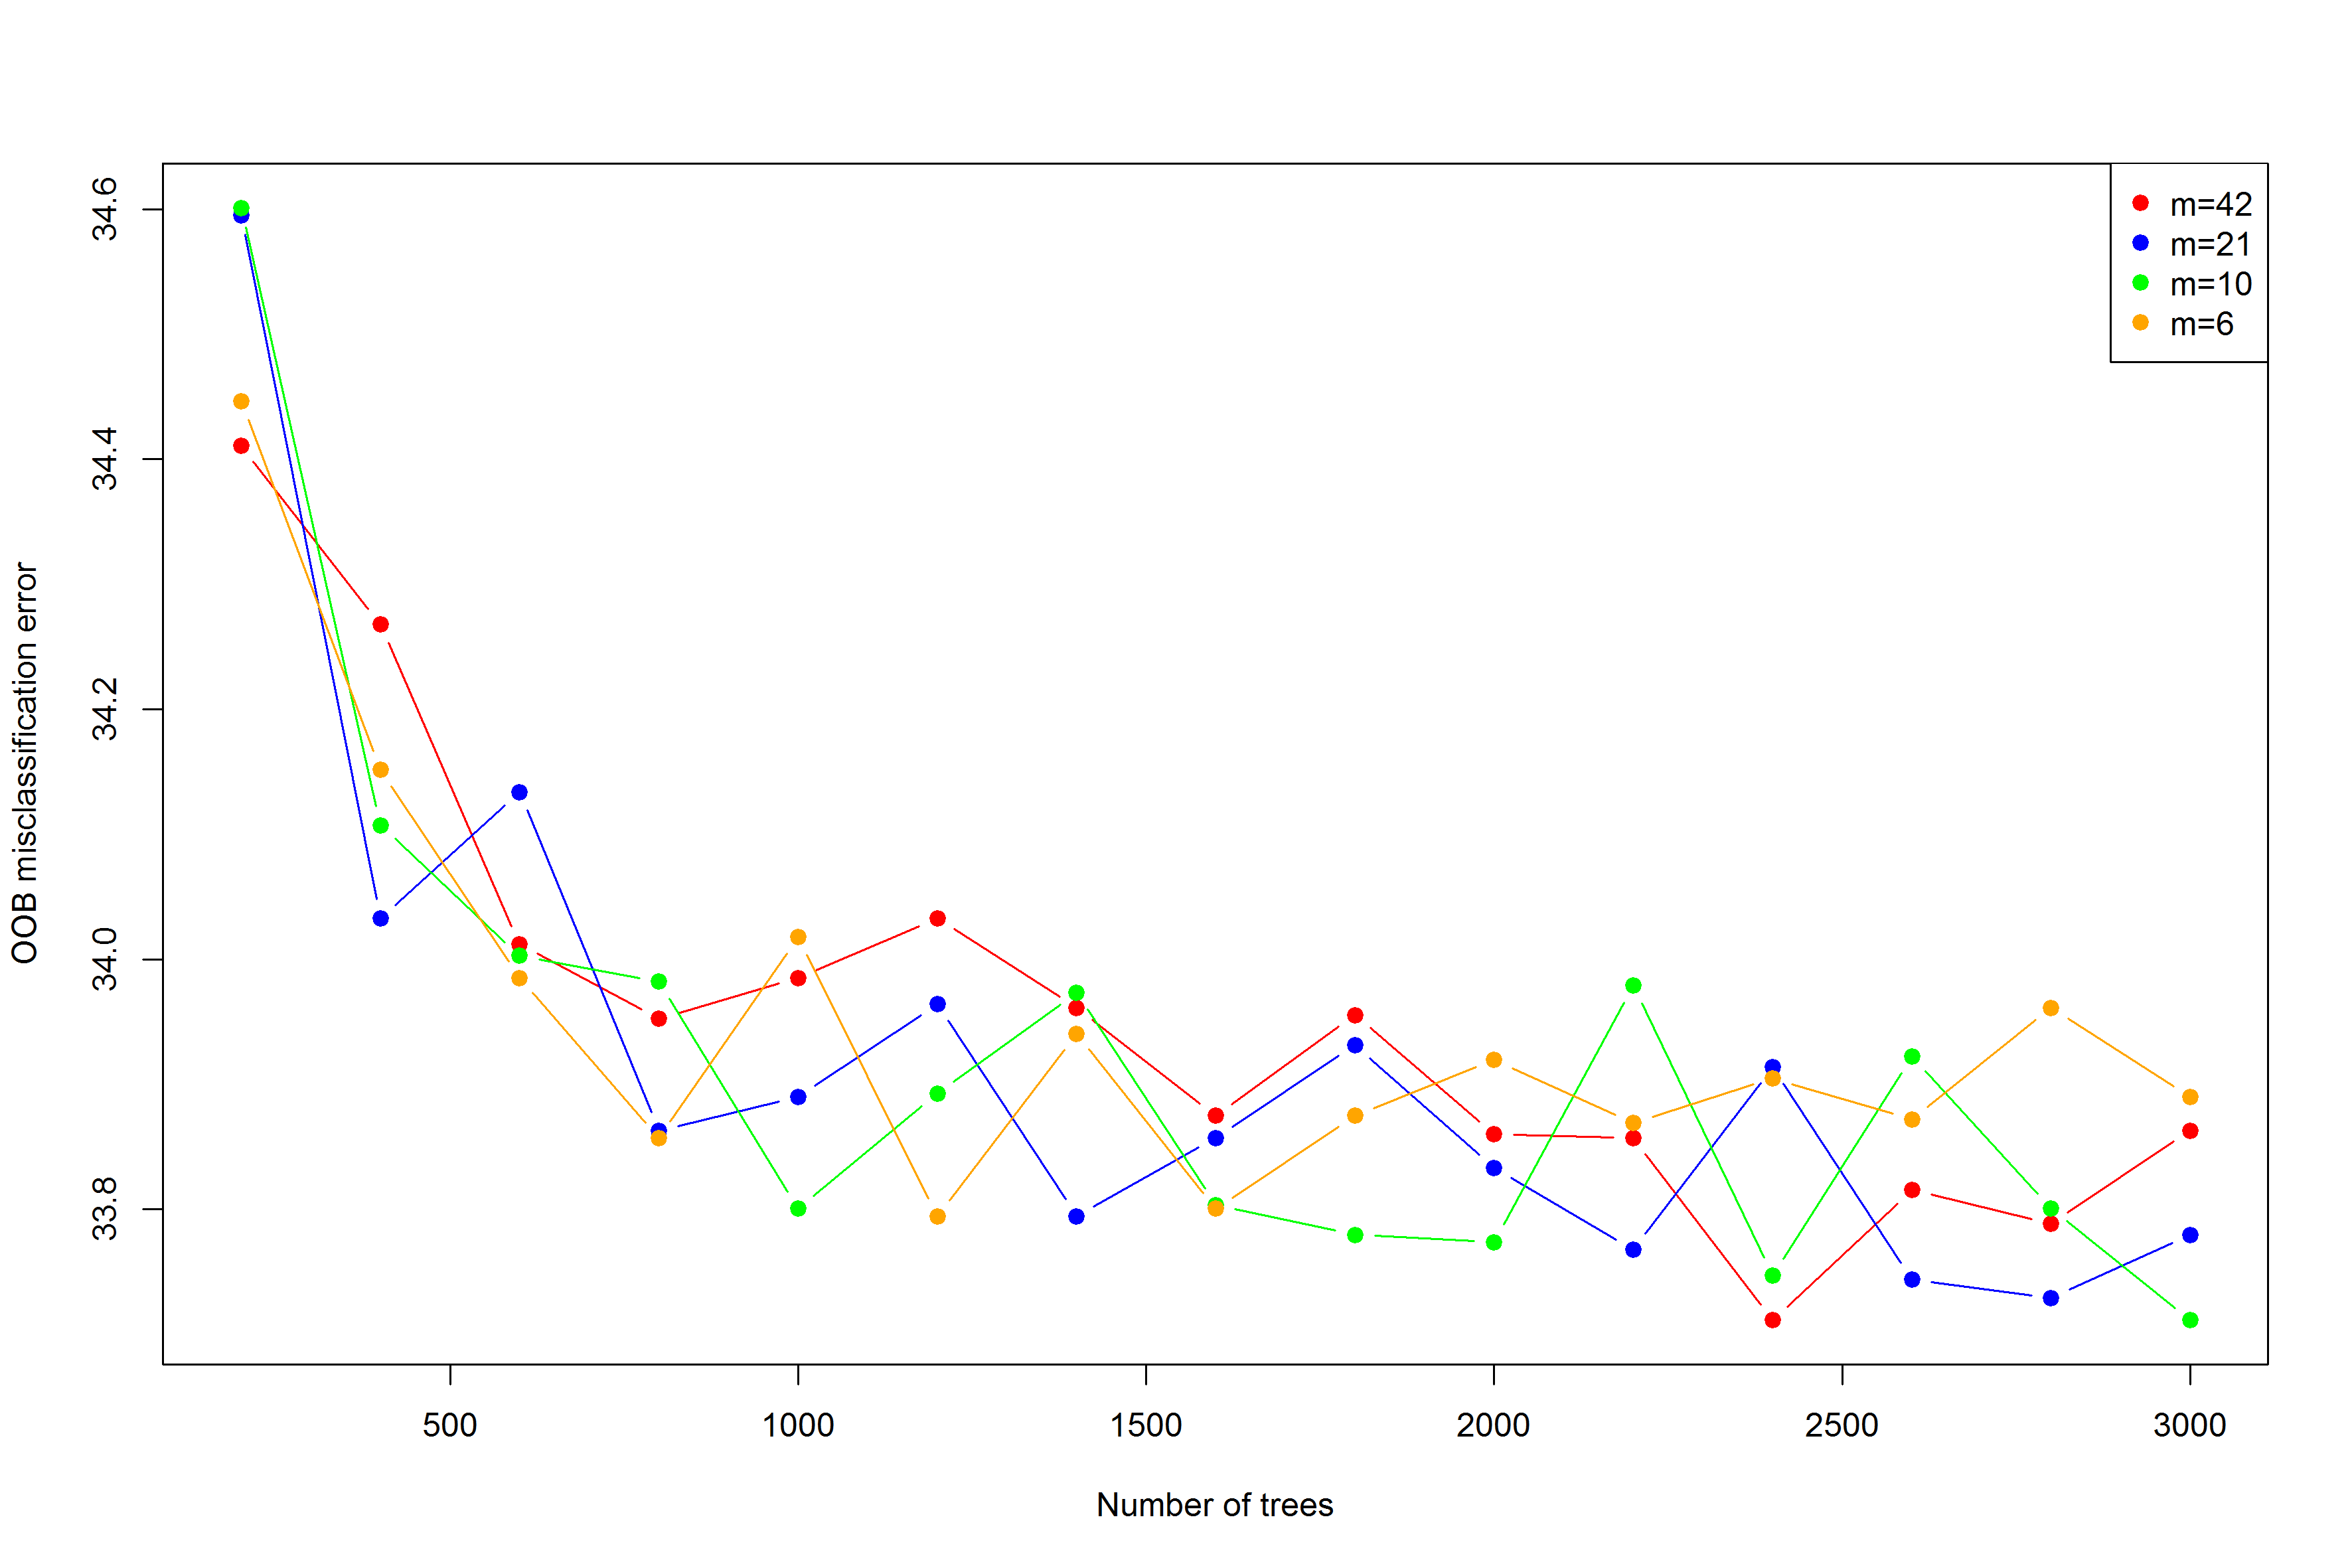
\includegraphics[width=0.9\linewidth]{img/300dpi/Fig_tree_depth_and_ntrees} 

}

\caption{Determining the optimal depth and the of number the trees in the random forest model.}\label{fig:tree_depth}
\end{figure}

\hypertarget{res}{%
\section{Association between time series features and AF/AD
performance}\label{res}}

Since the RF consists of a large number of trees, it is no longer
possible to represent the resulting statistical learning procedure using
a single tree, and it is not clear which variables are most important to
the procedure \citep{james2013introduction}. Therefore, the RF improves
prediction accuracy at the expense of interpretability. Instead, it is
possible to obtain the overall summary of the importance of each feature
by measuring the mean decrease in the Gini index.

\begin{figure}[H]

{\centering 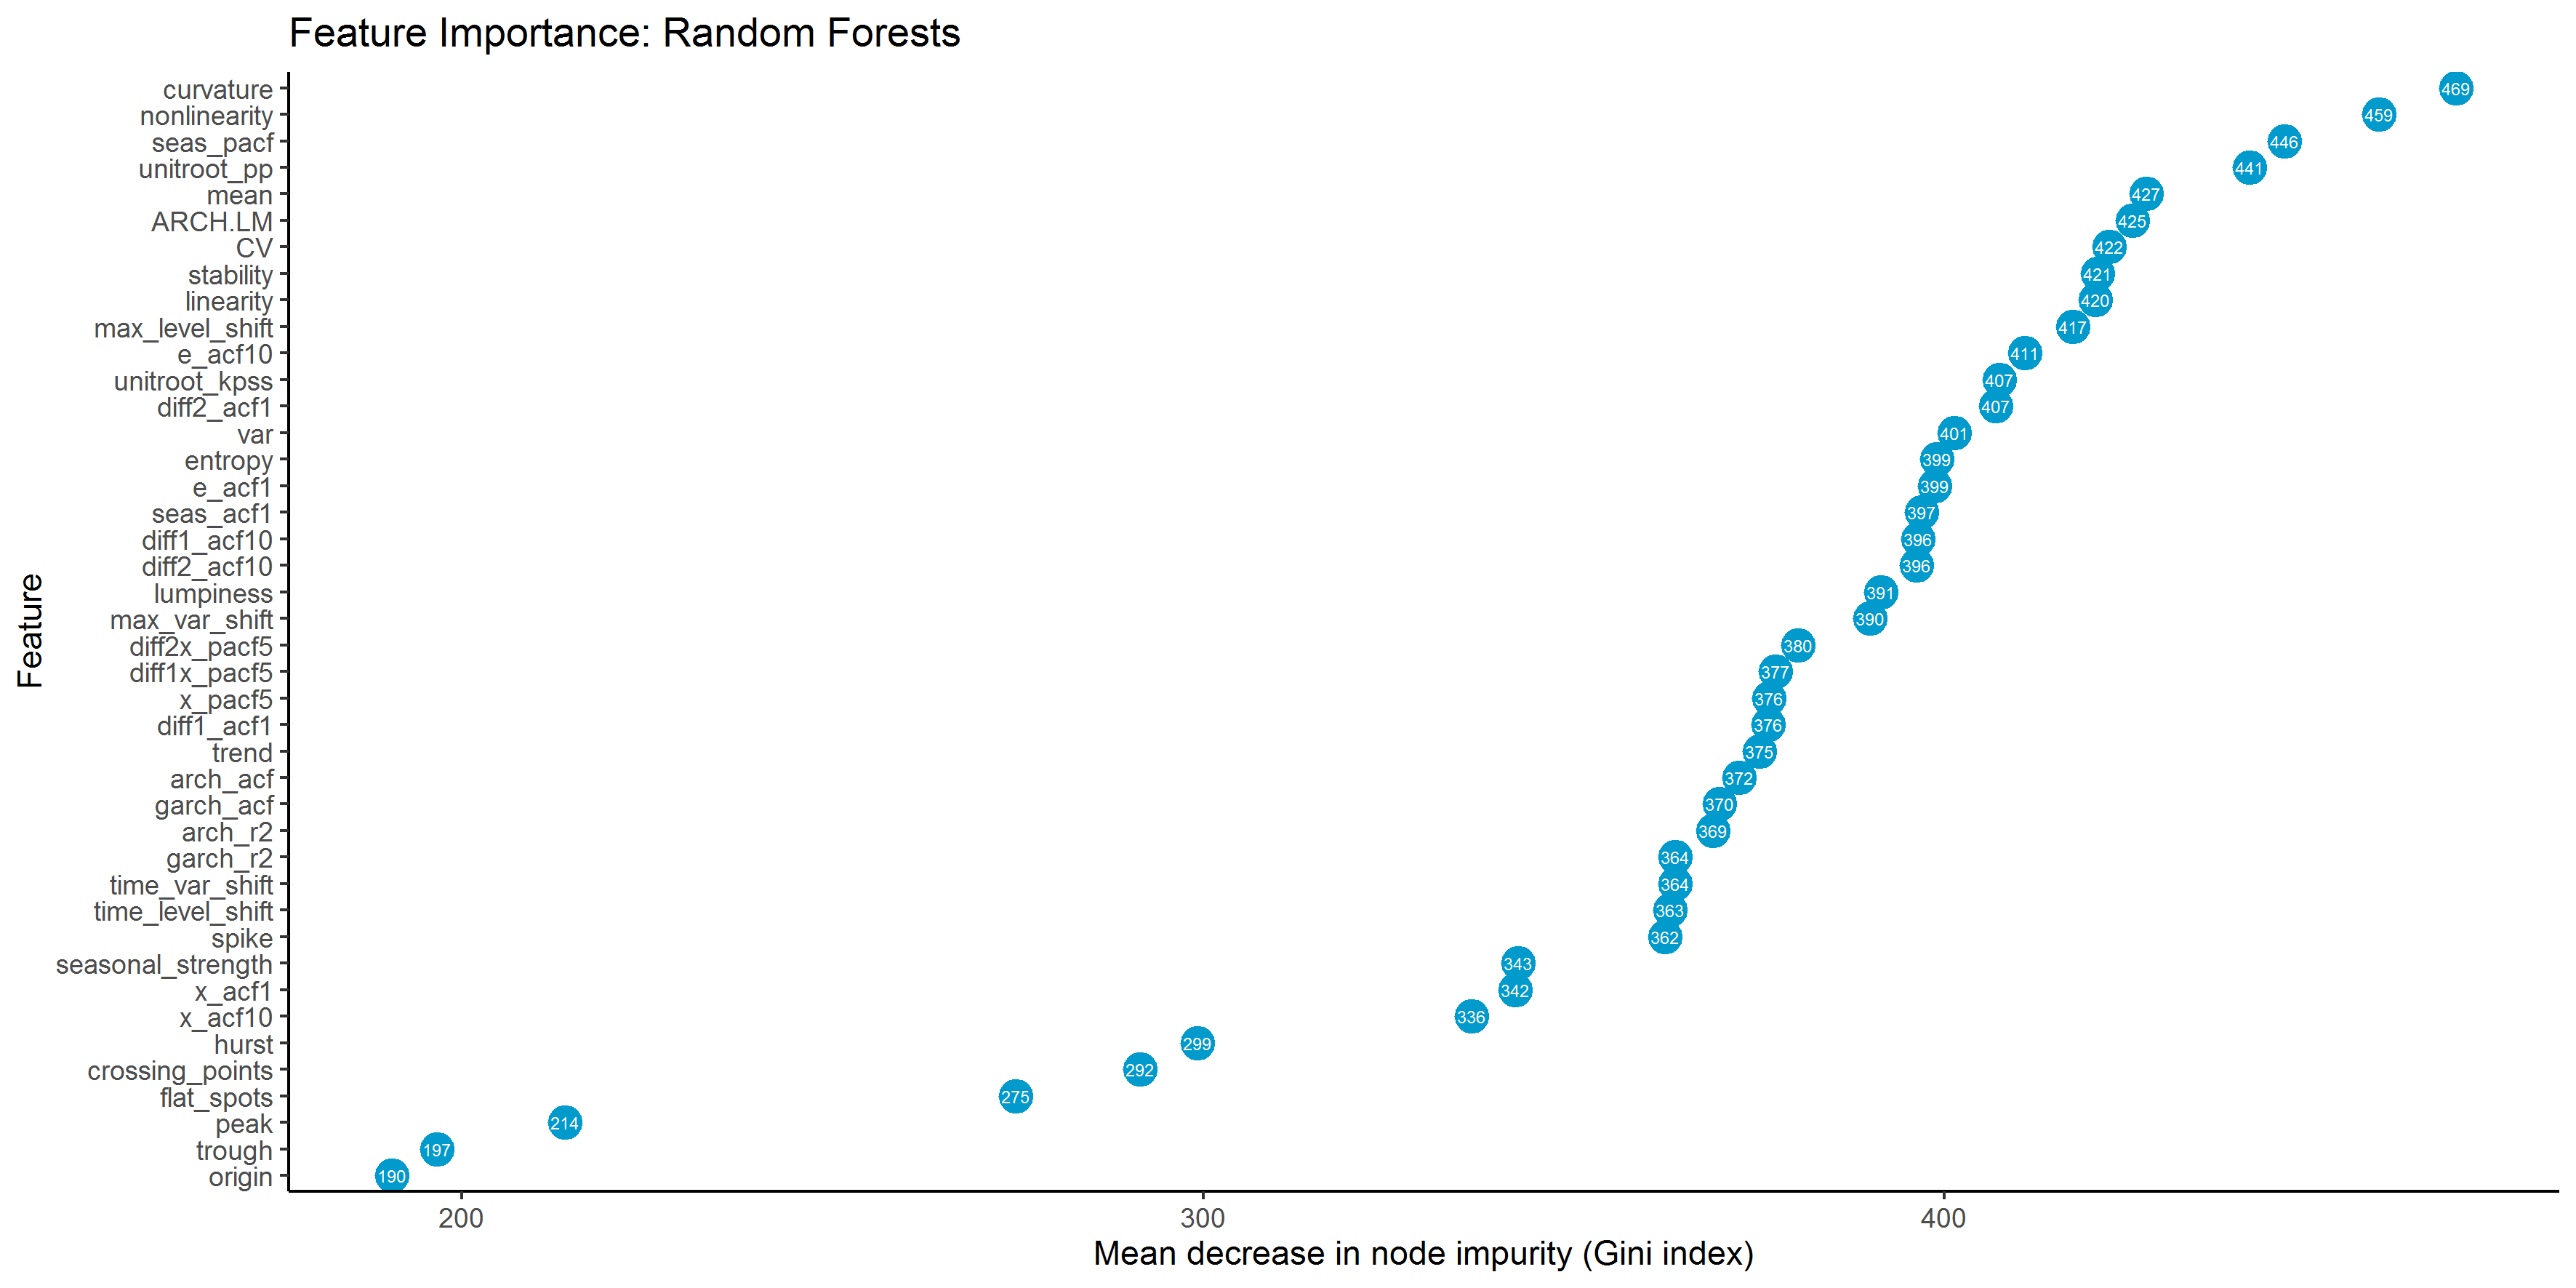
\includegraphics[width=0.95\linewidth]{img/300dpi/Fig_importance} 

}

\caption{Predictor features importance spectrum for the M4 data. A feature importance is computed using the mean decrease in Gini index.}\label{fig:RFpartial}
\end{figure}

The Figure \ref{fig:RFpartial} demonstrates the overall importance of
the features used in building trees during the random successive process
of generating the RF model. Importance of the features is determined by
the decrease in total amount of the node impurity by splits over a given
predictor and averaging over all trees in RF. The decrease of the node
impurity is measured by the Gini index. A large values of the Gini index
indicates the important features. Clearly some features prove to be more
important than others in classifying accurately the AF versus AD
approach. The most important features are: \emph{curvature},
\emph{nonlinearity}, \emph{seas\_pacf}, \emph{unitroot\_up}, \emph{mean}
and \emph{ARCHM.LM}; while \emph{origin}, \emph{through}, \emph{peak}
and \emph{flats spots} seems to be the least important for predicting
which temporal aggregation method to use (i.e.~AF or AD). The quantity
being modeled here is the probability of correctly choosing the AD
versus AF, and the opposite. The least important features have
approximately half of the importance as the most significant ones.
Difference in a decrease of node impurity from the \emph{curvature} to
the \emph{origin} feature is more than 250 units, indicating the wide
range of features importance.

\begin{figure}[H]

{\centering 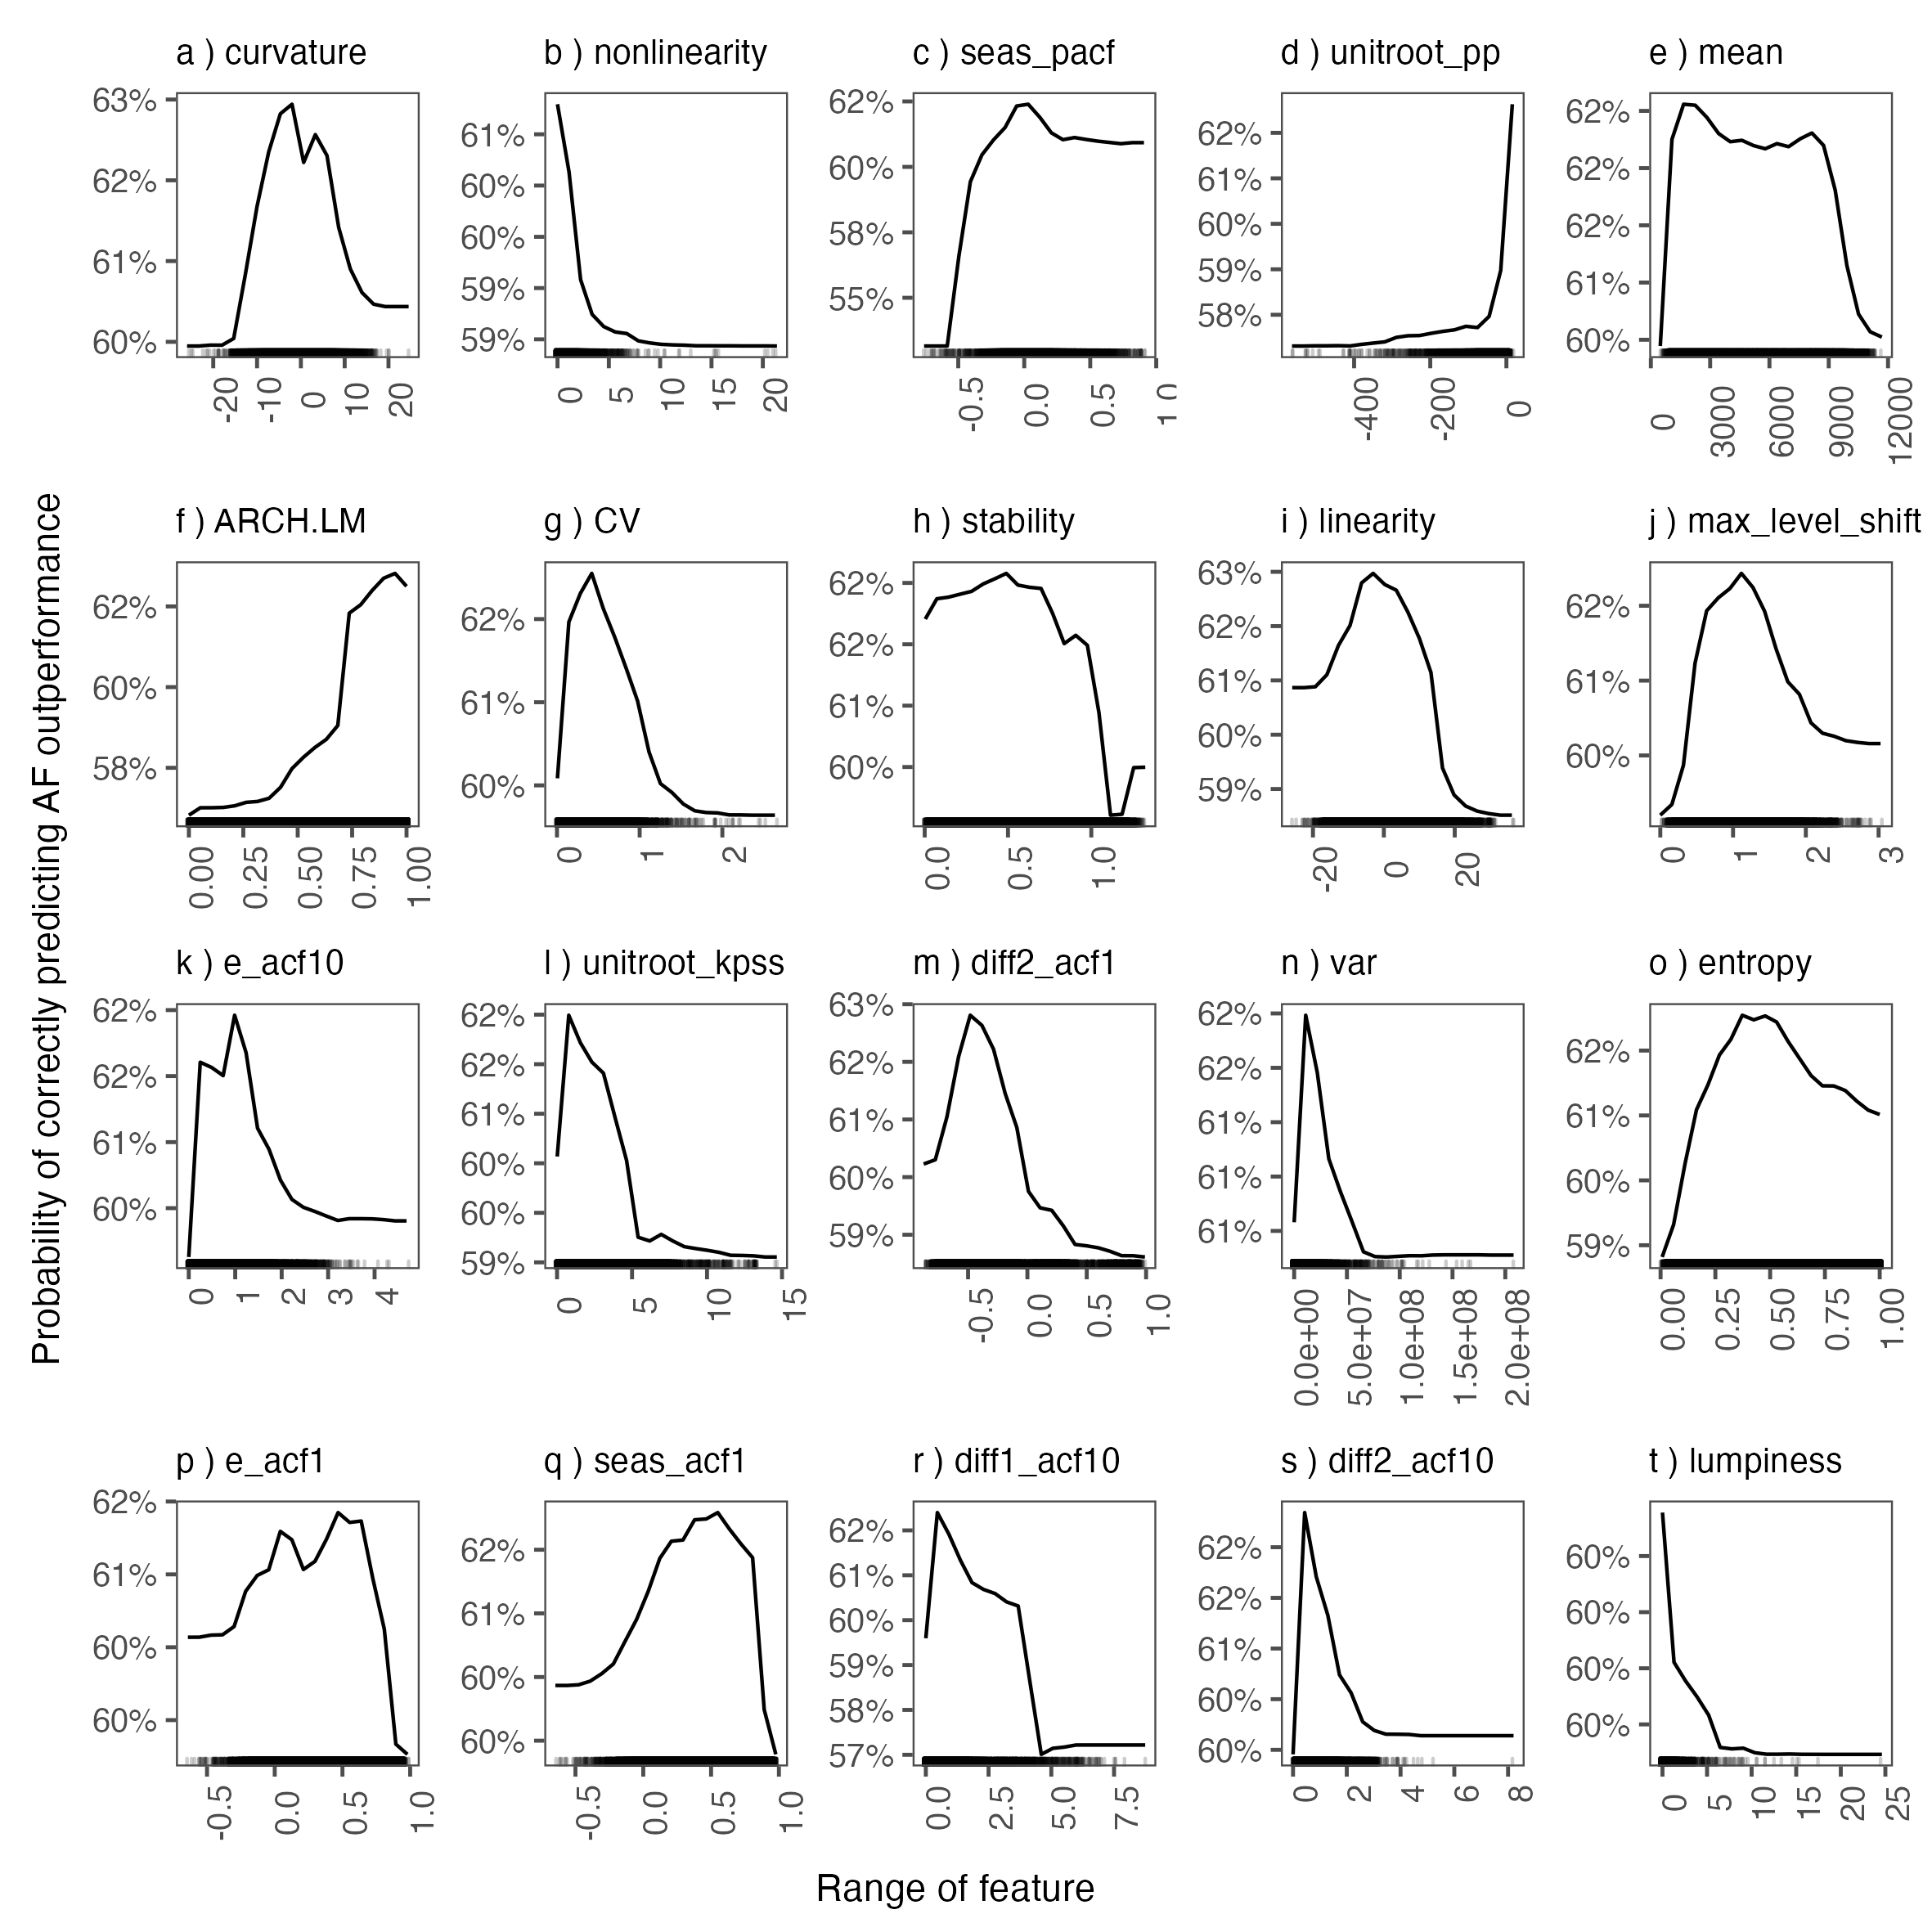
\includegraphics[width=1\linewidth]{img/300dpi/partial_dependence1} 

}

\caption{   extcolor{blue}{Partial dependence plot - the range of features vs. the probability of classifying AF versus AD} }\label{fig:pdpcommon1}
\end{figure}

\begin{figure}[H]

{\centering 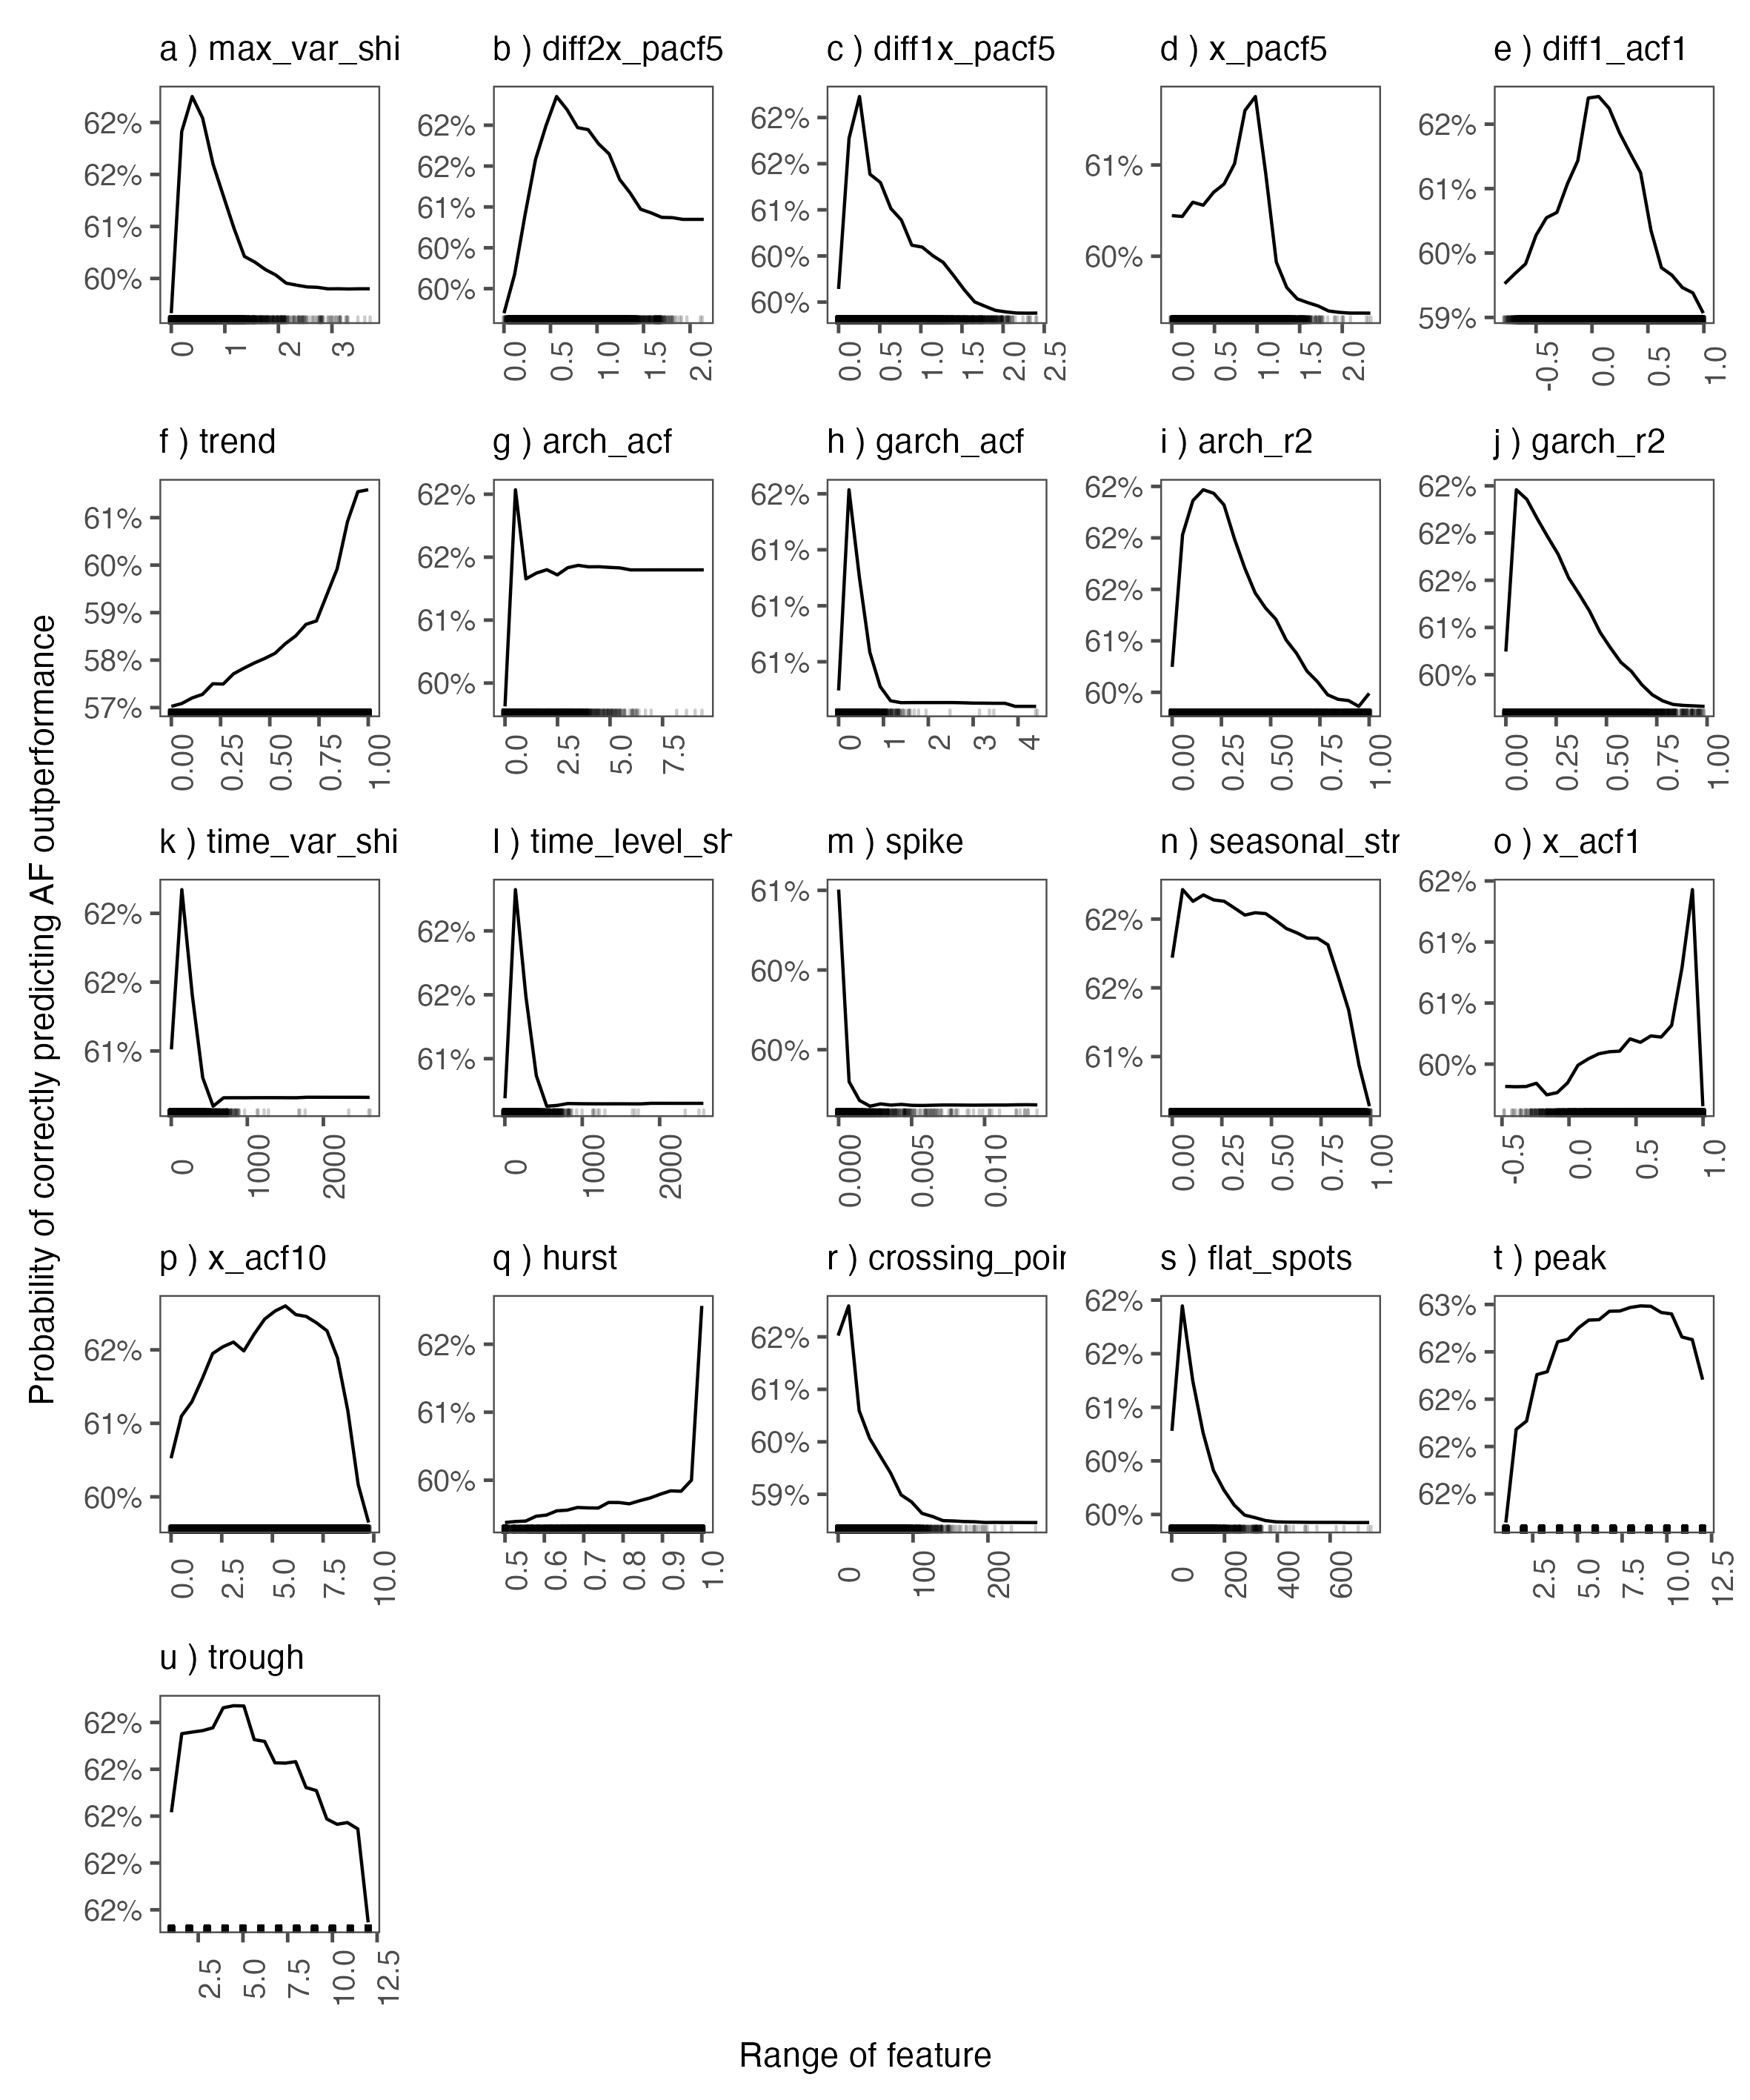
\includegraphics[width=1\linewidth]{img/300dpi/partial_dependence2} 

}

\caption{   extcolor{blue}{Partial dependence plot - the range of features vs. the probability of classifying AF versus AD (continue)} }\label{fig:pdpcommon2}
\end{figure}

Figure \ref{fig:pdpcommon1} and \ref{fig:pdpcommon2} represent the
partial dependence plot for all features.
\textcolor{blue}{The x-axis represents the range of values extracted for each feature and the y-axis is the probability of classifying AF versus AD. Therefore, the dependent value is the probability of correctly predicting the aggregating forecasts i.e. AF approach.}

The plots illustrate the marginal effect of the selected features on the
response (outcome) after integrating out all the other variables and
their average effect on the response \citep{james2013introduction}.

The rug marks at the bottom of each plot show the distribution of
feature across the variable range. Note that here the data density is
lower near the edges. This may cause unstable behavior of the curves in
those areas. The vertical scales of the plots show the probability of AF
approach providing more accurate forecast for each feature as values of
that feature changes. From Figure \ref{fig:pdpcommon1} and
\ref{fig:pdpcommon2}, it is clear that the features have a mixed effect
on classifying AF and AD approaches. While the effect might be clear for
feature such as trend or nonlinearity, it is less clear for other such
as mean or coefficient of variation.

We observe that increasing trend, ARCH.LM, hurst, autocorrelation lag 1,
unitroot\_pp and seas\_pacf may increases the chance of AF performing
better, therefore AF become preferable. However, increasing lumpiness,
entropy, nonlinearity, curvature, strength of seasonality may increase
the chance of AD performing better, so the strong presence of these
features may favorite AD over AF. It is important to note that we are
less interested in the exact probability in these plots. Instead, we are
interested in discovering how changing time series feature may
increase/decrease the chance of AF or AD.

\hypertarget{con}{%
\section{Conclusions}\label{con}}

In time series forecasting, a forecast time granularity required to
inform a decision, might be different from the time series granularity
itself. For instance, if a time series is stored at a higher frequency
(e.g.~monthly), forecasts might be required at a lower frequencies
(e.g.~quarterly, annual). This is very common in modern organisations as
data can be collected in the finest time granularities. Therefore, there
are situations where a forecast of the total value over
\textcolor{blue}{a time period} ahead (e.g.~horizon
aggregation/lead-time) is needed. To generate such a forecast for a
given time series, we may consider two options: i) first generate
forecasts, followed by adding them up to obtain the forecast horizon
aggregation (AF), or ii) first aggregate the time series using
non-overlapping temporal aggregation and then generate the forecast
(AD). In this paper, we design and execute an empirical experiment
framework using the monthly M4 competition data to i) explore the
forecasting performance of these approaches; and ii) investigate the
association between time series features and forecasting performance of
temporal aggregation approaches (e.g.~AF or AD).

There is a common assumption that series at the higher level of temporal
aggregation (lower frequency) are smoother with less noise and more
cleaner patterns, which often implies that forecasts created at the
higher temporal aggregation levels are more accurate. This practice may
exist in supply chains, where practitioners are usually advised to
aggregate the series to the frequency levels aligned with their decision
making horizons and then to create forecast for the period of interest.
In this paper, we questioned this practice and explore the comparative
performance of AF and AD approaches. We conducted a comparative research
of the forecasting performance using 48,000 monthly series from M4 data,
at different levels of temporal aggregation corresponding to generating
forecasts at bi-monthly, quarterly, 4--monthly, semi-annual and annual
levels. Results demonstrate that there is a significant number of series
for which aggregate forecast (63\%) outperforms aggregate data (37\%).

Given the fact that there is a lack of rules and indications on which
approach should be used for a given time series, we further investigate
the association between time series features and AF/AD forecasting
performance. The need for such a research investigation has also been
highlighted in the literature \citep{babai2022demand}. Therefore, we
seek to shed lights on the effect of temporal aggregation on time series
features and further investigate how they might affect the performance
of AD and AF approaches. To that end, we first construct a database
consisting of features of each time series as predictor and model class
labeled as AF/AD as response/outcome. Then, we build several ML models
to accurately predict the correct class and consequently recommend using
the most accurate approach for a given time series and its features.

Our results show that Random Forest model provides the best performance
in accurately classifying approaches measured through statistical and
utility metrics. Moreover, RF model is used to reveal the most important
time series features in producing the accurate prediction. Additionally,
we extract the partial dependence plot to describe the contribution of
time series features through a probability.
\textcolor{blue}{This helps to show how the value of a feature may favor AF over AD approach}.
The main findings of this study can be summarised as follows:

\begin{itemize}
\item
  First of all, when a forecast of the total value over several time
  periods ahead is required (i.e.~aggregation horizon or lead-time), we
  show that AF is a significantly better methodology to use overall. The
  findings indicate that neither of the approaches are always the most
  accurate, when the accuracy is reported for the individual time
  series. The findings clearly show that the most accurate forecast is
  not necessarily generated by non-overlapping temporal aggregation.
  This may call into question the justification of the common practice
  in such a situation.
\item
  Second, non-overlapping temporal aggregation changes the features of
  time series. The magnitude of the change varies for different
  features. In particular, we observe that with increase in the
  aggregation level, the strength of seasonality, the autocorrelation,
  coefficient of variation, linearity, curvature and KPSS unitroot
  statistic decrease. However, nonlinearity, mean, variance, ARCH.LM,
  trend , unitroot pp statistics increase. Entropy is the only measure
  that both increases and decreases based on its initial value.
\item
  Third, Random Forest model is the most accurate classifier ML
  algorithm in predicting which approach provides more accurate forecast
  given a set of time series features as input.
\item
  Fourth, RF model revels that the top ten important features for
  predicting whether AF or AD should be used for a given monthly time
  series in M4 competition include \emph{curvature},
  \emph{nonlinearity}, \emph{seas\_pacf}, \emph{unitroot\_up},
  \emph{mean}, \emph{ARCHM.LM}, \emph{Coifficient of Variation},
  \emph{stability}, \emph{linearity} and \emph{max\_level\_shift}.
\item
  Fifth, dependence plots provide some indications on how time series
  features may favorite AD over AF, vice-versa. We observe that
  increasing seas\_pacf, trend, ARCH.LM, hurst, autocorrelation lag 1
  and unitroot\_pp increases the chance of AF performing better. While,
  increasing Coefficient of Variation, entropy, nonlinearity, curvature
  increases the chance of AD performing better, so the strong presence
  of these features may favorite AD over AF.
\end{itemize}

\textcolor{blue}{The proposed framework can be generalised to be used with other time series data. We believe that the conclusion should remain true for lower frequency time series such as monthly and quarterly. However, a different conclusion might be reached when using higher frequency time series data such sub-daily, daily, or weekly. This will bring further complications such as the presence of multiple seasonal cycles and long seasonalities. Therefore, time series features and the way they may change with increasing the aggregation level may differ. Also, the choice of forecasting method becomes important as a method like ETS cannot handle those complications. This would be an important avenue for further research.}

Given the findings of this study and the potential value of temporal
aggregation in time series forecasting, the current study could be
extended in a number of ways. Research into any of the following areas
would prove to be useful:

\begin{itemize}
\item
  In this study, we use all features to build the ML model, an
  alternative approach would be to use dimension reduction approaches
  for all features representing the same type of information such as
  seasonality, autocorrelation, noise, etc and then build the model;
\item
  \textcolor{blue}{The proposed framework can be used to examine the association of time series features and temporal aggregation with sub-daily and daily time series data as they present further complications.}
\item
  \textcolor{blue}{Given that the exact relationship between time series features and the optimal temporal aggregation approach is not known, one direction for future research could focus on using meta-learning and other advanced techniques such as transformers neural networks and attentional mechanism to further shed lights on this problem.}
\item
  \textcolor{blue}{In this paper, we define the AD and AF approaches to forecast a cumulative number of periods ahead, therefore it is considered as a single output approach. It might be interesting to investigate the forecasting by temporal aggregation as a multi-output scenario [@de2022data], where a sequence of two or more future data points are of interest.}
\item
  \textcolor{blue}{Finally, using time-series classification techniques [@buza2018time] to classify time series data based on various factors including time series futures and investigate their association with forecast accuracy of temporal aggregation approaches might be also an interesting avenue for further research.}
\end{itemize}

\hypertarget{reproducibility}{%
\section*{Reproducibility}\label{reproducibility}}
\addcontentsline{toc}{section}{Reproducibility}

R code and RMarkdown file to produce all results in this paper are
available at
\url{https://github.com/bahmanrostamitabar/time-searies-featute-temporal-aggregation}

\hypertarget{appendix}{%
\section*{Appendix}\label{appendix}}
\addcontentsline{toc}{section}{Appendix}

\begin{landscape}\begin{table}[!h]

\caption{\label{tab:modelSetup}The main setup information for ML models}
\centering
\resizebox{\linewidth}{!}{
\fontsize{8}{10}\selectfont
\begin{tabular}[t]{>{\raggedright\arraybackslash}p{1cm}>{\raggedright\arraybackslash}p{2cm}>{\raggedright\arraybackslash}p{1cm}>{\raggedright\arraybackslash}p{1cm}>{\raggedright\arraybackslash}p{6cm}>{\raggedright\arraybackslash}p{3cm}>{\raggedright\arraybackslash}p{3cm}}
\toprule
Model & R package & Running time (min) & Feature enginering & Activation formula & Optimization algorithm & Main assumptions and limitations\\
\midrule
LR & stats & \textasciitilde{}3 & NO & glm(marks\textasciitilde{}.,family = binomial, data=train.data) & maximum likelihood estimation & linear relationship between the response and the predictor variables\\
LDA & MASS & \textasciitilde{}3 & NO & lda(marks\textasciitilde{}., data=train.data) & singular value decomposition & normally distributed data and equal covariance class matrices\\
QDA & MASS & \textasciitilde{}3 & NO & qda(marks\textasciitilde{}., data=train.data) & maximum likelihood estimation & normally distributed data\\
KNN & class & \textasciitilde{}20 & YES & knn(Xlag[train,], Xlag[-train,], ClassTable[train,"marks"], k=3) & grid search & sensitive to the choice of the hyperparameter k\\
LASSO & glmnet & \textasciitilde{}10 & NO & cv.glmnet(x, y, family="binomial", type.measure="auc") & coordinate descent method & linear relationship between the response and the predictor variables\\
GAM & gam & \textasciitilde{}12 & NO & gam(marks\textasciitilde{}. + s(trend, df=3) + s(seas\_acf1, df = 3) + s(linearity, df = 3) + s(entropy, df = 3) + s(x\_acf1, df = 3) + s(seasonal\_strength, df = 3) + s(seas\_acf1, df = 3), family = binomial, data = train.data) & penalized regression maximum likelihood estimation & additive relationship between the predictor variables and the response variable\\
RF & randomForest & \textasciitilde{}2200 & NO & randomForest(marks\textasciitilde{}., data=train.data1, mtry=10, ntree=3000, importance = TRUE) & bootstrap aggregation & parsimony, overfitting, interpretability and long computation time\\
Boosting & gbm & \textasciitilde{}3000 & YES & gbm(marks\textasciitilde{}., data = train.data01, distribution = "bernoulli", n.trees = 4500, shrinkage = 0.01, interaction.depth = 10) & gradient boosting & parsimony, overfitting, interpretability and long computation time\\
SVM & e1071 & \textasciitilde{}6000 & YES & tune(e1071::svm, as.factor(marks)\textasciitilde{}., data = train.data, scale = FALSE, kernel = "radial", ranges = list(cost=c(0.001 , 0.01, 0.1, 1, 5, 10, 100), gamma=c(0.5, 1, 2, 3, 4))) & Lagrange multipliers for constrained optimization problem & interpretability, sensitivity to kernel choice, assumes that the classes can be separated by a linear boundary or a hyperplane in high-dimensional space, long computation time\\
FNN & nnet & \textasciitilde{}10 & YES & nnet(marks\textasciitilde{}., data=train.data, size=10, maxit=500, decay=0.001, rang = 0.1) & resilient backpropagation algorithm & interpretability, limited flexibility, choice of hyperparameters and overfitting\\
DTW & dtw & \textasciitilde{}5 & YES & knn(train = trainData[, -5], test = testData[, -5], cl = trainLabels, k = k, prob = TRUE, use.all = TRUE, distance = dtw.dist) & dynamic programming algorithm & interpretability, computational complexity, sensitivity to noise and choice of warping function\\
DL Torch & torch & \textasciitilde{}180 & YES & nn\_module(  "Net",  initialize = function() \{  self\$fc1 <- nn\_linear(length(features1), 40),  self\$fc2 <- nn\_linear(40, 30),  self\$fc3 <- nn\_linear(30, 30), self\$fc4 <- nn\_linear(30, 15),  self\$fc5 <- nn\_linear(15, 15),  self\$fc6 <- nn\_linear(15, 10), self\$fc7 <- nn\_linear(10, 10),  self\$fc8 <- nn\_linear(10, 5),  self\$fc9 <- nn\_linear(5, 5),  self\$fc10 <- nn\_linear(5, 1) \},
  forward = function(x) \{  x \%>\% 
      self\$fc1() \%>\%  nnf\_relu() \%>\%  self\$fc2() \%>\% nnf\_relu() \%>\% self\$fc3() \%>\%  nnf\_relu() \%>\% self\$fc4() \%>\% nnf\_relu() \%>\% self\$fc5() \%>\% nnf\_relu() \%>\% self\$fc6() \%>\%      nnf\_relu() \%>\%  self\$fc7() \%>\%  nnf\_relu() \%>\%  self\$fc8() \%>\%  nnf\_relu() \%>\% self\$fc9() \%>\%  nnf\_relu() \%>\% self\$fc10() \}) & adaptive moment estimation & interpretability, computational complexity, choice of hyperparameters, overfitting and long computation time\\
XG Boost & xgboost & \textasciitilde{}300 & YES & xgboost(data = xgboost\_train, max.depth=23, nrounds=500, objective = "binary:logistic") & gradient boosting with decision trees & interpretability, computational complexity, choice of hyperparameters, overfitting and long computation time\\
TensorFlow & tensorflow, keras & \textasciitilde{}30 & YES & keras\_model\_sequential() \%>\% layer\_dense(units = 80, activation = "relu", input\_shape = c(42)) \%>\%  layer\_dropout(rate = 0.6) \%>\%  layer\_dense(units = 40, activation = "relu") \%>\%  layer\_dropout(rate = 0.3) \%>\%  layer\_dense(units = 5, activation = "relu") \%>\%   layer\_dense(units = 1, activation = "sigmoid") & root mean square propagation & interpretability, computational complexity, choice of hyperparameters and overfitting\\
RNN & keras & \textasciitilde{}30 & YES & keras\_model\_sequential() \%>\%  layer\_lstm(units = 64, input\_shape = c(42, 1)) \%>\%  layer\_dropout(rate = 0.2) \%>\%  layer\_dense(units = 1, activation = "sigmoid") & adaptive moment estimation & temporal dependence between the input and output variables, interpretability, computational complexity, choice of hyperparameters and overfitting\\
CNN & keras & \textasciitilde{}35 & YES & keras\_model\_sequential() \%>\%  layer\_conv\_1d(filters = 32, kernel\_size = 3, activation = "relu", input\_shape = c(42, 1)) \%>\%  layer\_max\_pooling\_1d(pool\_size = 2) \%>\%
layer\_dropout(rate = 0.2) \%>\%  layer\_flatten() \%>\%  layer\_dense(units = 1, activation = "sigmoid") & adaptive moment estimation & spatial dependence between the input and output variables, interpretability, computational complexity, choice of hyperparameters and overfitting\\
\bottomrule
\end{tabular}}
\end{table}
\end{landscape}

\renewcommand\refname{References}
\bibliography{mybibfile.bib}


\end{document}
